
% DEBE TENER DOS O TRES P�GINAS. NO MENOS, NO M�S

% Compilalo con pdflatex
\documentclass[a4paper, 11pt]{article}
  %\usepackage[dvips]{graphicx}
  \usepackage[pdftex]{color,graphicx}
  \newif\ifpdf
    \ifx\pdfoutput\undefined
      \pdffalse % we are not running PDFLaTeX
    \else
      \pdfoutput=1 % we are running PDFLaTeX
    \pdftrue \fi
  \ifpdf
  \usepackage{url}
  % RELLENAR
    \usepackage[pdftitle={},
                pdfauthor={},
                pdfsubject={},
                pdfkeywords={},
  	      pdfproducer={pdfLaTeX}
                pdftex,
                colorlinks=true,
                linkcolor=blue,
                pdfstartview=FitH]{hyperref}
  \pdfcompresslevel=9 \else
    \usepackage{hyperref}
  \fi


  \usepackage[utf8]{inputenc}
  \usepackage[spanish]{babel}
  \usepackage{verbatim}
  \usepackage{makeidx}
  \usepackage{calc} % para que funcione bien \ojo{}
  \usepackage{shadow}
  \usepackage{xspace}
  \usepackage{graphicx}
  \usepackage{subfigure}
  \usepackage{enumerate}
  \graphicspath{ {img/} }
  %
  % Para opciones de men
  %
  \newcommand{\menu}[1]{\fbox{#1}}
  \newcommand{\pestanya}[1]{pestanya\fbox{#1}}
  \newcommand{\boton}[1]{boton\fbox{#1}}
  \newcommand{\flecha}{\ensuremath{\Rightarrow}}

  % Estas longitudes estuvieron activas hasta el 1 Julio 2001, en que pase'
  % al formato de fancyheadings
  %\addtolength{\textheight}{5cm}
  %\addtolength{\textwidth}{4cm}
  %\addtolength{\oddsidemargin}{-2cm}
  %\addtolength{\evensidemargin}{-2cm}
  %\addtolength{\topmargin}{-3cm}


  %%%%%%%%%%%% Inicio de cabecera y pie de pagina %%%%%%%%%%%%%%%%%%%%%%%%%
  \usepackage{fancyheadings} % para cabeceras y pies de pagina
  \pagestyle{fancyplain}
  %%%%%
  \voffset -1cm
  \hoffset -0.5cm
  \oddsidemargin  0pt
  \evensidemargin 0pt
  \textwidth 16.5cm
  \addtolength{\textheight}{3.5cm} % alargar longitud p�ina
  % ensanchar cabecera de p�ina
  \addtolength{\headwidth}{\marginparsep}
  \addtolength{\headwidth}{\marginparwidth}
  \addtolength{\headwidth}{2cm}

  \renewcommand{\sectionmark}[1]{\markright{#1}{}}
  %\lhead[\fancyplain{\bfseries\thepage}{\bfseries\thepage}]
  \lhead[\fancyplain{\sl\footnotesize\bfseries\rightmark}{\sl\footnotesize\bfserie
  s\rightmark}]
  {\sl\footnotesize\fancyplain{\bfseries\rightmark}
  {\sl\footnotesize\rightmark}}
  \rhead[\fancyplain{\sl\bfseries\thepage}{\sl\bfseries\thepage}]
  {\fancyplain{\sl\bfseries\thepage}{\sl\bfseries\thepage}}
  \cfoot{}


  %%%%%%%%%%%%%%%%%%%%%%%%%%%%%%%%%%%%%%%%%%%%%%%%%%%%%%%%%%%%%%%%%%%%%%%
  %
  % Caja para avisos de cosas que faltan por corregir, por ejemplo
  % (sacada de elec-pot.tex, y mejorada para ajustar automaticamentewww.
  % el ancho de la caja)
  %
  \newcommand{\ojodos}[1]{ } % Comentar para ver dudas adicionales
  \newcounter{numeroOjo}\setcounter{numeroOjo}{0}
  \def\anchoColumnaReal{\columnwidth-\marginparsep-\marginparwidth}
  \newcommand{\ojo}[1]{%
  \begin{center}%
    \setcounter{numeroOjo}{\value{numeroOjo}+1}
    \shabox{\parbox{\anchoColumnaReal}{{\bf Ojo!!!}: (\thenumeroOjo) #1}}
  \end{center}}
  %
  % Crear una caja de texto con borde para destacar ciertos parrafos
  %
  \newcommand{\destacaP}[1]{%
  \begin{center}%
    \shabox{\parbox{\anchoColumnaReal}{#1}}
  \end{center}}


  %\makeindex

  %
  % Guiones de separacion de palabras
  %
  \hyphenation{Su-pon-ga-mos re-co-men-da-ble}

  \begin{document}

  \title{\emph{Anteproyecto Trabajo Fin de Grado} \\
   Aplicacion para moviles inteligentes para el deporte\\
   Application for smartphone for sport\\
  }
  \author{
   Director \\ David Santo Orcero - \url{correo:dsanto@lcc.uma.es} \\ \\
   Alumno \\ Rubén Gutiérrez Cazorla - \url{correo:gutyruben@gmail.com}\\ \\
   Departamento \\Lenguajes y Ciencias de la Computación
   }
  \maketitle


  \thispagestyle{empty}
  %\newpage
  %\tableofcontents
  %\newpage

  %%%%%%%%%%%%%%%%%%%%%%%%%%%%%%%%%%%%%%%%%%%%%%%%%%%%%%%%%%%%%%%%%%%%%%%%%%%%%%%%%%%%%%%%%%%%%%%
  %
  %
%


\section{Introducción}

      En los últimos años, los móviles han sufrido un rápido avance que aún no hemos
      asimilado. La llegada de internet a estos realizo un gran salto y posteriormente
      el salto a los smartphone. Con ellos hubo un cambio de paradigmas: en la forma
      de comunicarnos, de comprar, alimentarnos y como no: también la forma de hacer
      deporte.\\

      Con la llegada del GPS a nuestros móviles nos han aportado una gran herramienta
      para ser utilizada para mapas y poder llegar a sitios de una manera sencilla.
      Por otro lado se puede utilizar desde un enfoque más deportivo y usarse para una
      medición precisa de nuestros entrenamientos.\\

      Realizar una aplicación para dispositivos móviles que permite registrar todas
      tus actividades deportivas: vía GPS, con ella podemos tener un historial y
      seguimiento de todas nuestras actividades, como: correr, caminar, ciclismo y
      mucho más.\\

      Para llevar el control de nuestras actividades realizamos un seguimiento de
      ciertos parámetros como: la distancia, tiempo, calorías quemadas, velocidad,
      altitud y mucho más.\\

      Con el registro de podremos llevar un control sencillo de las actividades y
      progresar con interesantes datos y estadísticas.\\

      Para los que quieren ponerse en forma de manera sencilla, hacer ejercicio,
      adelgazar corriendo, empezar a correr con un asistente personal, terminar esa
      maratón o hacer carreras populares.\\

      La principal funcionalidad de la aplicación es la medición del ejercicio,
      deportivo realizado. Donde el usuario antes de iniciar la actividad, necesitará
      iniciar la aplicación y en la primera vista, pulsar un botón, el cual activará
      la funcionalidad GPS y comenzará a realizar un seguimiento. El conjunto de las
      ubicaciones GPS y el tiempo en el que realiza la actividad, nos dará como
      resultado la velocidad. También se podrá obtener otras datos como las calorías
      (aproximadas) quemadas en dicho entrenamiento. Esto quedará almacenado en la
      memoria del teléfono para poder usar los datos.\\

      Dicha base de dato ha de ser lo más liviana posible, puesto que no todos los
      terminales disponen de una gran capacidad y con la arquitectura que más se
      adecue en relación: espacio/velocidad*.\\

      *Dicha relación se refiere al espacio que ocupa la base de dato y la velocidad
      que tenga de transmisión de la información.\\

      En otra vista tendremos una lista de ejercicios deportivos realizados por el
      usuario, donde podrá visualizar los entrenamientos realizados, ordenados por
      fecha, siendo la última realizada la primera en aparecer. También contendrá
      datos relevantes del entrenamiento como: distancia recorrida, tiempo y calorías
      quemadas, entre otros. Para ello nos apoyaremos en las bases de datos.\\

      Enfocado para el usuario que quiera afinar más en el campo de la quema de
      grasas, tendremos una vista que permita introducir: su peso, sexo, altura y
      edad. Con estos tres parámetros y gracias a la fórmula de Harris-Benedict, es la
      que vamos a utilizar para calcular la cantidad de calorías quemadas, y se
      calcula de la siguiente manera:

      \begin{itemize}
        \item{Mujeres:  [655 + (9.6 x Peso kg) ] + [ (1.8 x Altura cm) – (4.7 x Edad)] x Factor actividad}
        \item{Hombres:  [66 + (13.7 x Peso kg) ] + [ (5 x Altura cm) – (6.5 x Edad)] x Factor actividad}
      \end{itemize}
        \\Cuando se nombra factor de actividad se refiere a lo siguiente:
      \begin{itemize}
        \item{Personas sedentarias (hace poca actividad física): 1.2}
        \item{Actividad ligera (hace actividad física 1 a 3 veces por semana): 1.375}
        \item{Actividad moderada (hace actividad física 3 a 5 veces por semana): 1.55}
        \item{Actividad intensa (hace actividad física 6 a 7 veces por semana): 1.725}
        \item{Actividad extremadamente alta (atletas profesionales mucha actividad física): 1.9}
      \end{itemize}

      Esta actividad irá de la mano del historial que tengas en la vista antes
      mencionada. Y no se incluirá el factor actividad en la vista en la que tenemos
      la listas de los ejercicios realizados si no que se usará para la vista que
      mencionamos a continuación.\\

      Por último y no menos importante una vista en la que nos proporciona el
      resultado de todo el trabajo realizado, y el cálculo total de calorías quemadas,
      usando el factor actividad, puesto que ya sabremos cuantas veces a la semana se
      está realizando la actividad.\\



\section{Estado del arte}

    \subsection{Introducción}





      Para poder comenzar a hablar de nuestra aplicación y sus beneficios tenemos
      que entender que es la actividad fisica. Pues según la OMS "la actividad
      física cualquier movimiento corporal producido por los músculos esqueléticos
      que exija gasto de energía." También nos indica los factores que provocan
      la mortalidad mundial y de cómo una actividad regular tiene efectos
      beneficiosos en la salud y previene numerosas enfermedades.\\

      %http://www.who.int/dietphysicalactivity/pa/es/

      En la actualidad vivimos en una sociedad que ha ido añadiendo poco a poco
      una actividad deportiva en sus vidas, además de una alimentación sana. Sin
      importar lo que los mueve ya sea sobre peso, una busqueda más profesional
      del ejercicio físico o para encontrarse bien, encuentran comoda una
      aplicación que supervise su progreso. \\

      Como observamos, en el libro Anuario de Estadisticas deportivas 2016,
      perteneciente al Ministerio de educación, Cultura y Deporte y editada por
      la Secretaría General de Documentación y Publicaciones, observamos
      distintos indicadores de aumento en la realización de actividades
      deportivas, si lo hacemos desde un punto de vista empresarial observamos
      en la siguiente tabla como hay un aumento de actividades deportivas en
      empresas vinculadas al deporte por actividad económica:\\

      \begin{figure}[H]
          \centering
          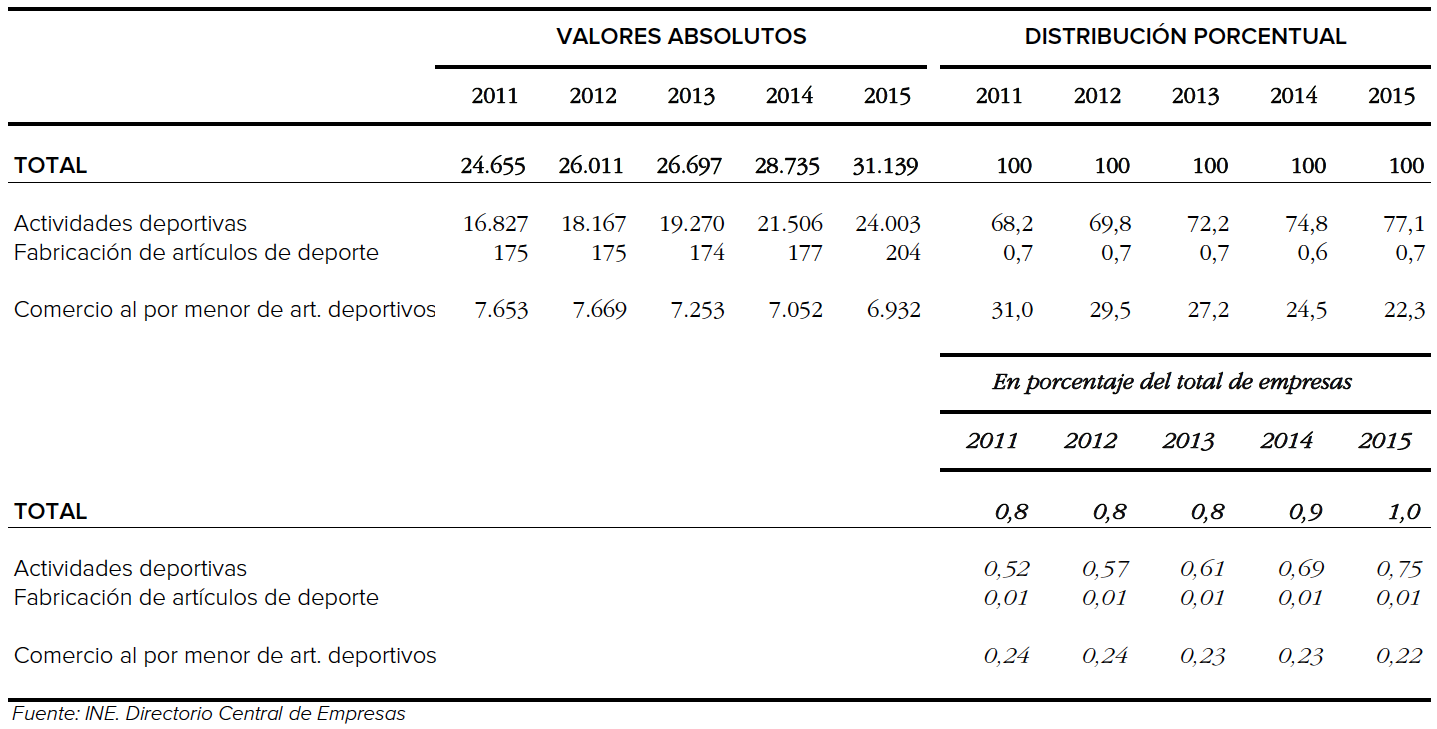
\includegraphics[width=1\textwidth]{empresas-vinculadas-al-deporte-por-actividad-economica}
          \caption{Empresas vinculadas al deporte por actividad económica}
          \label{f:empresas}
      \end{figure}

      Como vemos en la figura (\ref{f:empresas}) existe un incremento desde el
      año 2011 al 2015 de actividades deportivas. Ergo si las empresas ven un
      incremento en sus actividades deportivas esto significa que hay una demanda
      de las misma siendo un indicador de un aumento te usuarios que realizan
      actividades deportivas.\\

      Otro gran indicativo, más directo que el de las empresas vinculadas al
      deporte por actividad económica, es la información relativa al gasto de
      consumo de los hogares.\\

      \begin{figure}[H]
          \centering
          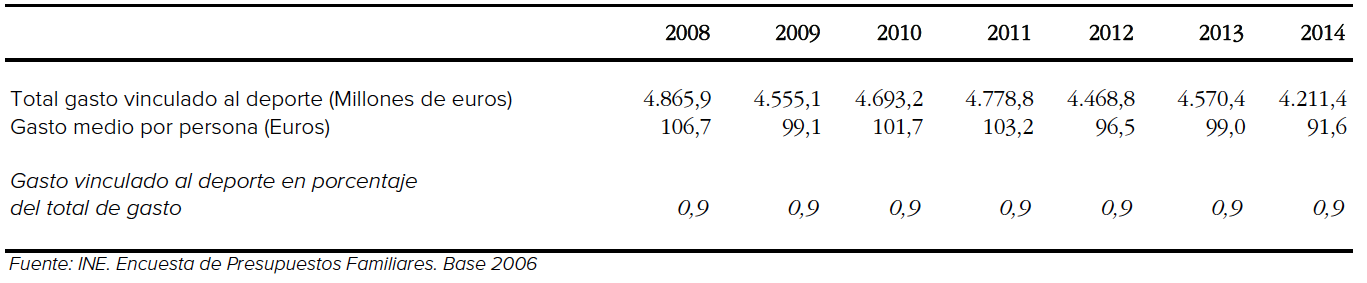
\includegraphics[width=\textwidth]{Gasto-en-bienes-y-servicios-vinculados-al-deporte}
          \caption{Gasto en bienes y servicios vinculados al deporte}
          \label{f:hogares}
      \end{figure}

      En esta figura (\ref{f:hogares}) nos muestra una disminucion del gasto
      vinculado al deporte, pero teniendo en cuenta que el esutido se realiza en
      un periodo que abarca desde el 2008 al 2014 y teniendo en cuenta "En
      diciembre de 2008 la economía entró en recesión y consiguió salir de ella
      en mayo de 2010, aunque por poco tiempo ya que el PIB siguió cayendo en
      tasa interanual hasta que en abril de 2012 encadenó dos trimestres
      consecutivos de descensos y España volvió a entrar en recesión." (Periodico
      La Razón: http://www.larazon.es/economia/fechas-clave-de-la-crisis-economica-en-espana-CX4077260).
      Pero este gaston no tiene porque influir en la actividad deportiva sin costo
      como puede ser correr o el ciclismo y teniendo en cuenta que la cantidad
      no dismunuye considerablemente se deduce que aún en tiempos de desdicha
      económica se mantiene esa cultura del deporte.\\

      Centrandonos en la población española la información relativa a los habitos
      y prácticas deportivas desde una edad de 15 años en adelante.\\

      \begin{figure}[H]
          \centering
          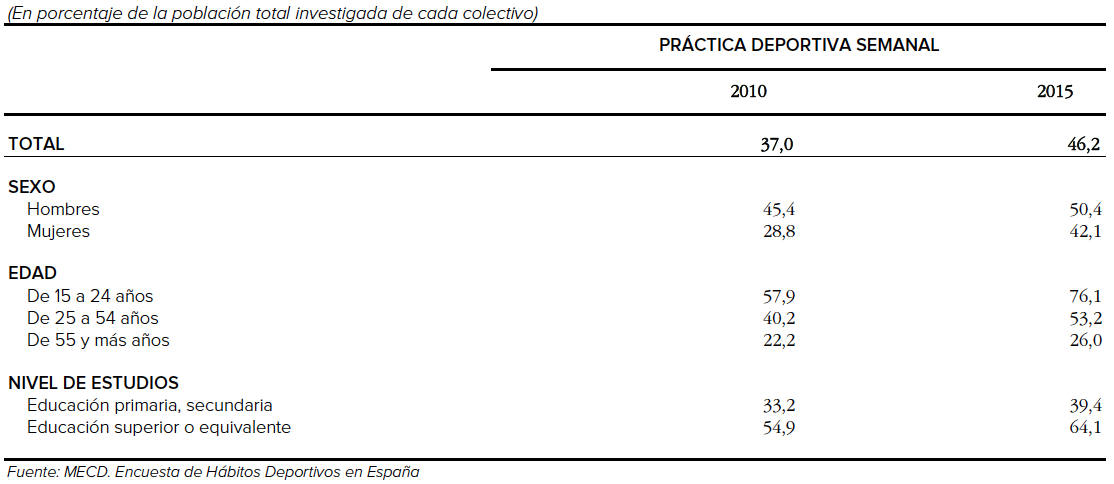
\includegraphics[width=1\textwidth]{Personas-que-practican-deporte-semanalmente-segun-caracteristicas-personales}
          \caption{Personas que practican deporte semanalmente según características personales}
          \label{f:personas}
      \end{figure}

      En la figura (\ref{f:personas}) se observa que en cuanto al deporte
      practicado en 2015 es superior al 2010 con una diferencia de 9,2 \% de la
      población. Siendo las Mujeres las que más se han lanzado a la realización
      de deporte. En cuanto a la edad comprendida entre 15 y 24 años este aumento
      a supuesto 18,2\%. Siendo unos indicadores más que importantes para lanzar
      una aplicación para dispositivos moviles, pues este sector es el que más
      interiorizado tiene estas tecnologías.\\

      Paremos un momento para analizar el estado actual de la sociedad española
      en el campo de la tecnología. En cuanto a la cantidad de la población adulta
      que tiene algún tipo de movil es del 96\%, haciendonos ver que hay una
      normalidad en nuestra sociedad al uso de telefonos pero lo mas llamativo
      es que el estudio nos muestra un 80\% de la población con telefonos
      inteligentes. Entre las acciones que realizamos los españoles nos
      encontramos en primer lugar tenemos con un 51\% aplicación de mensajería,
      un 38\% para reproducir vídeos, en cuanto a la cifra mas baja tenemos con
      un 25\% el uso para jugar, por otro lado tenemos a las finanzas con un
      33\% y por último tenemos con un 39\% de la población que usa servicios de
      mapas en sus dispositivos móviles. Como nos explica XatakaMovil (En:
      https://www.xatakamovil.com/movil-y-sociedad/espana-territorio-smartphone).\\

      Como resumen tenemos que en "2015 el 53,5\% de la población de 15 años en
      adelante practicó deporte en el último año. La mayor parte de ellos, el
      86,3\%, con gran intensidad, al menos una vez a la semana. Los resultados
      muestran que un 70,6\% de la población suele realizar esta actividad y el
      68,2\% al menos una vez por semana. Respecto al hábito de andar y su
      relación con la práctica deportiva, un 81,1\% de la población manifiesta
      que suele andar o practicar deporte semanalmente. La encuesta investiga
      asimismo tanto la asistencia." (dicho en en el libro Anuario de
      Estadisticas deportivas 2016).\\

      % aunario de estadísticas deportivas 2016
      Tambie existen datos que nos indica que hay una parte de ella la cual
      es obesa, como estima el boletin de la OMS en que existe un tanto
      porciento de esta poblacion practica de porte un tanto por ciento a la
      semana por lo tanto la relevancia de la aplicacion es mas que
      significativa por una ayuda del control de los datos viologicos del sujeto
      en la practica deportiva\\

      Según "Las recomendaciones mundiales sobre la actividad fisica para la
      salud" escritas por la OMS y nos muestra tres grupos acotados en función
      de la edad, desde niños a ancianos y a cada grupo se le introduce un
      minimo de tiempo, tipo de actividad e intensidad de la misma. Con el fin
      de evitar lesiones cardíacas, mejora de la musculatura.\\

      Hay que tener en cuenta que no podemos darle la misma actividad fisica a
      todos los usuarios y eso es fundamental. Lo que podemos sacar de este
      estudio es que todos necesitamos una actividad fisica adecuada a nuestro
      momento\\

      \begin{comment}

              La evolución de los dispositivos electrónicos personales, ha desembocado
              en una fuerte presencia de teléfonos móviles, más concretamente Smartphone.
              El cual nos ayuda en nuestra vida cotidiana. La facilidad de acceder a
              un Smartphone y la simplicidad en la instalación de aplicaciones, hacen
              que sea un elemento inseparable. e. La historia de la telefonía móvil
              daría para crear otro trabajo de gran envergadura, pero es necesario
              mencionar el fenómeno del Smartphone. Si bien ya existían sistemas
              operativos para móviles como Symbian o BlackBerry, no fue hasta el 2007,
              con el lanzamiento al mercado del primer iPhone, y el 2008, con el
              lanzamiento del primer teléfono con el sistema operativo Android, el HTC
              Dream, que se empezó a utilizar este concepto para referirnos a nuestros
              teléfonos. Desde entonces, la popularidad y las ventas de ambos sistemas
              ha aumentado como la espuma, llegando a la situación que he mencionado
              antes, (Gartner: http://www.gartner.com/newsroom/id/3609817 ) donde
              Android tiene aproximadamente un 80.7 \% de las ventas de móviles, iOS un
              17.7, Microsoft con su Windows 10 Mobile 1.1 \%, BlackBerry con 0.2 \% y
              el 0.2 \% para otros sistemas operativos.\\

              Tras la aparición de los primeros sistemas operativos hubo una serie de
              evoluciones en los Smartphone que nos lleva hasta nuestros días. Cambios
              que supusieron un antes y un después y que nos lleva a la pieza angular de
              nuestro proyecto: El Sistema de Posicionamiento Global, mac conocido como:
              GPS. Pero ¿Qué es el GPS? Es un sistema que permite determinar en toda la
              Tierra la posición de un objeto con una precisión de hasta centímetros,
              aunque lo habitual son unos pocos metros de precisión. Este sistema se
              sirve de 24 satélites y utiliza la trilateración para saber de nuestra
              posición.\\

              %(Wikipedia https://es.wikipedia.org/wiki/Sistema_de_posicionamiento_global#Evoluci.C3.B3n_del_sistema_GPS ).

              El GPS ha sido el pilar de innumerables aplicaciones, algunas de ellas de
              manera indirecta para compartir nuestra localización y otras más directas,
              las cuales se basan en conocer cada ciertos segundos nuestra posición,
              para indicar una ruta desde un punto A, tu posición actual, a un punto B,
              donde quieres ir. Este TFG se basa en monitorizar tu posición vía GPS y
              obtener la distancia recorrida, gracias a un cronometro tener conocimiento
              del tiempo que tardas en realizar ese recorrido y obteniendo tu velocidad
              media, gracias a la ecuación v = e / t.\\

              Por otro lado y complementando a los cálculos anteriores esta el calculo
              de calorías quemadas Enfocado para el usuario que quiera afinar más en el
              campo de la quema de grasas, tendremos una vista que permita introducir:
              su peso, sexo, altura y edad. Con estos tres parámetros y gracias a la
              fórmula de Harris-Benedict, es la que vamos a utilizar para calcular la
              cantidad de calorías quemadas, y se calcula de la siguiente manera:

      \end{comment}

      Como inicio a las aplicaciones  y cerrando la introducción vamos a visualizar
      las aplicaciones y la cantidad de usuarios y descargas que hay:\\

      \begin{itemize}
        \item{Runtastic:}
        \begin{itemize}
          \item{"Runtastic hace público su número de usuarios: El éxito de la
                 compañía de salud y forma física móvil continúa y celebran 30
                 millones de descargas de sus apps, 25 millones de usuarios
                 móviles y 10 millones de usuarios registrados en el sitio
                 Runtastic fitness. Además lanza su línea de hardware en EEUU e
                 inicia una cooperación con Power Music." (https://www.socialetic.com/runtastic-25-millones-de-usuarios-y-una-descarga-de-su-app-cada-segundo.html)}
        \end{itemize}
      \end{itemize}
      \begin{itemize}
        \item{FITAPP GPS - Correr y Caminar:}
        \begin{itemize}
          \item{Tiene más de un millon de descargas (Dato aportado por Play Store)
                y la cantidad de usuarios es desconocida.}
        \end{itemize}
      \end{itemize}
      \begin{itemize}
        \item{Strava GPS Correr Ciclismo:}
        \begin{itemize}
          \item{Tiene más de diez millon de descargas (Dato aportado por Play Store)
                y la cantidad de usuarios es desconocida.}
        \end{itemize}
      \end{itemize}
      \begin{itemize}
        \item{RunKeeper - GPS Correr Caminar:}
        \begin{itemize}
          \item{Tiene más de diez millon de descargas (Dato aportado por Play Store)
                y la cantidad de usuarios es desconocida.}
        \end{itemize}
      \end{itemize}

    \subsection{Aplicaciones analizadas}

          \subsubsection{Runtastic}


              %   \includegraphics{{runtastic1}}\includegraphics{{runtastic2}}\includegraphics{{runtastic3}}\includegraphics{{runtastic4}}\includegraphics{{runtastic5}}\includegraphics{{runtastic6}}\includegraphics{{runtastic7}}




              \begin{figure}[H]
                  \centering
                  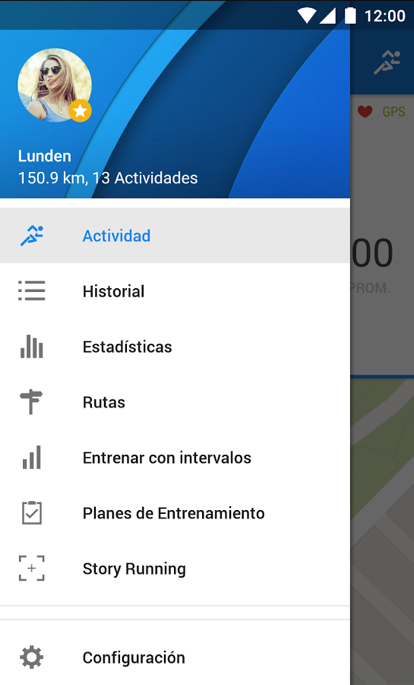
\includegraphics[width=0.3\textwidth]{runtastic1}
                  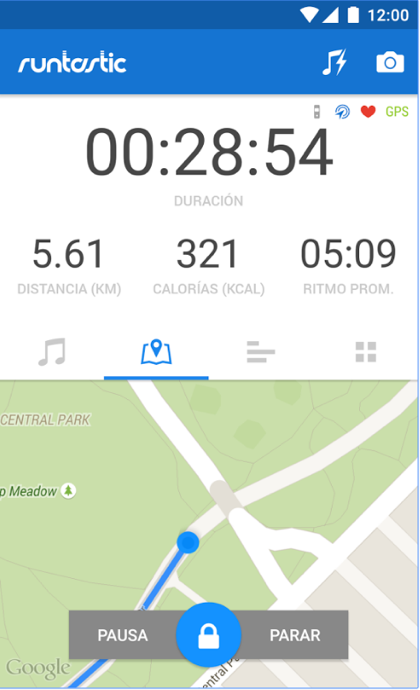
\includegraphics[width=0.3\textwidth]{runtastic2}
                  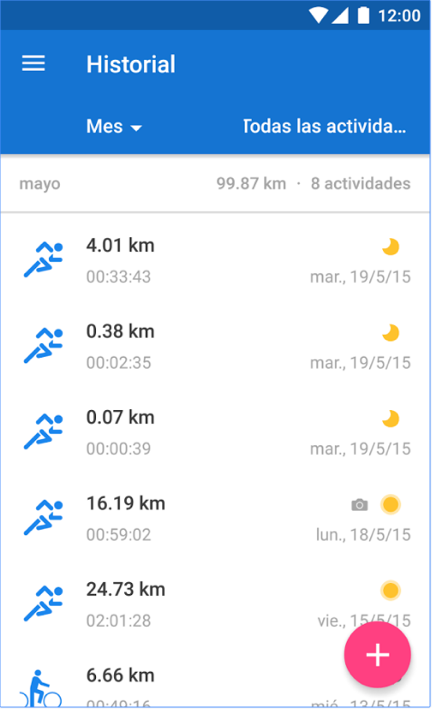
\includegraphics[width=0.3\textwidth]{runtastic3}
                  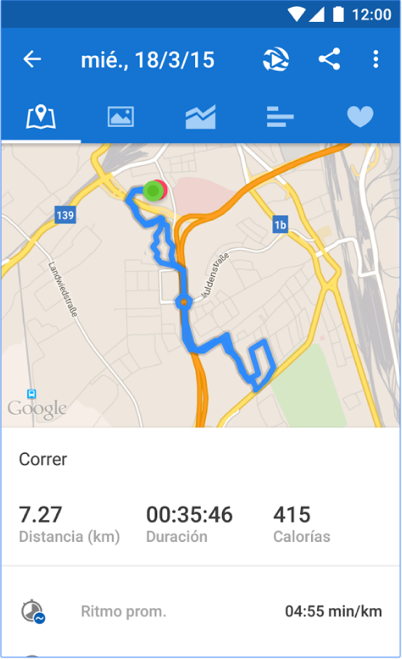
\includegraphics[width=0.3\textwidth]{runtastic4}
                  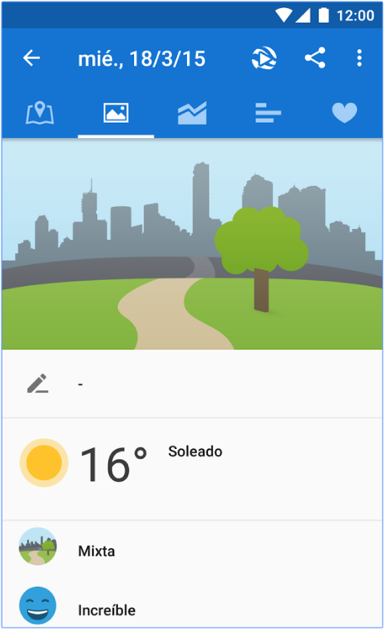
\includegraphics[width=0.3\textwidth]{runtastic5}
                  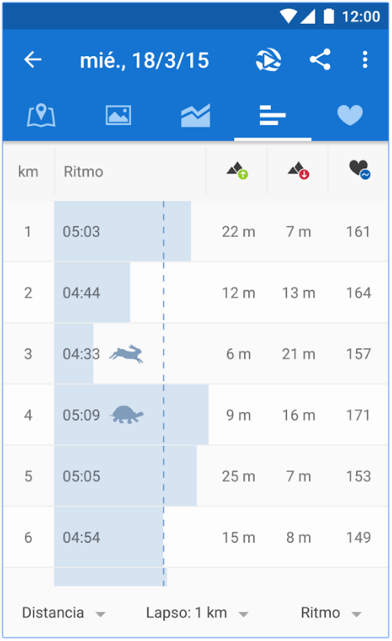
\includegraphics[width=0.3\textwidth]{runtastic6}
                  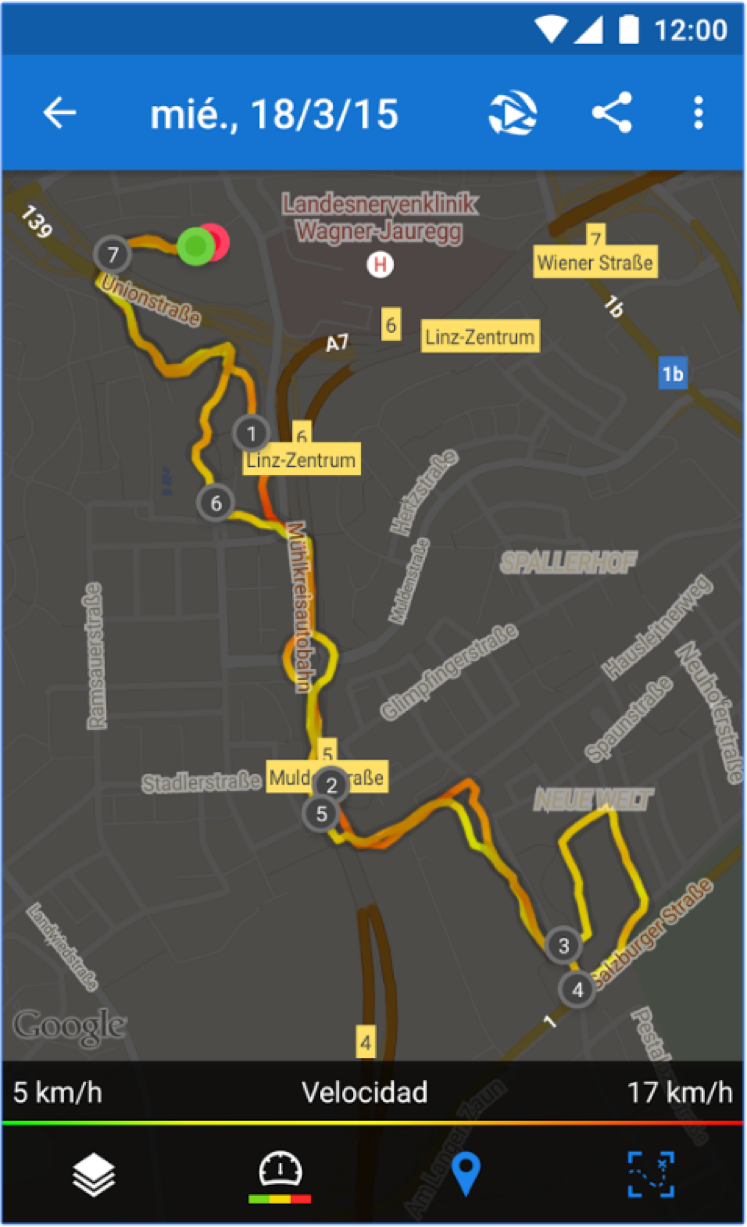
\includegraphics[width=0.3\textwidth]{runtastic7}
                  \caption{Múltiples imágenes de runtastic}
                  \label{f:runtastic}
              \end{figure}
              \\\\\textcolor[rgb]{1,0,0}{Aqui va la imagen: Imagenes runtastic}\\\\

                  \begin{itemize}
                    \item{FUNCIONES DE LA APP}
                    \begin{itemize}
                    	\item {Tu entrenador personal de running y fitness: correr, caminar, ir en bici, etc.)}
                    	\item {Entrenador por voz: tu entrenador personal te dice cómo lo vas haciendo según tus preferencias}
                    	\item {Android Wear 2.0: puedes dejar el móvil en casa y ver tus estadísticas en tu smartwatch}
                    	\item {Grupos: crea un grupo con tus amigos para motivaros}
                    	\item {Objetivo de running anual: ¡Ponte un objetivo! Si quieres empezar a correr o habituarte a hacer ejercicio, ¡aquí encontrarás tu motivación!}
                    	\item {Control de zapatillas: registra el kilometraje de tus zapatillas de running para que sepas cuándo debes cambiarlas por unas nuevas}
                    	\item {Clasificación: ¿te has propuesto adelgazar corriendo con tus amigos? ¡A ver quién puede correr más!}
                    	\item {Seguimiento y motivaciones en vivo: recibe mensajes de apoyo de tus amigos en vivo y en directo}
                    	\item {Powersong: reproductor de música integrado y powersong. ¡Así correr o caminar para ponerse en forma cuesta mucho menos!}
                    	\item {Runtastic Wearable Connect: las estadísticas de tus actividades, ahora en la pantalla de tu Runtastic Orbit o Runtastic Moment}
                    	\item {Integración con Google Fit y MyFitnessPal}
                    \end{itemize}
                  \end{itemize}

          \subsubsection{FITAPP GPS - Correr y Caminar}
              %   \includegraphics{{fitfapp}}
              \begin{figure}[H]
                  \centering
                    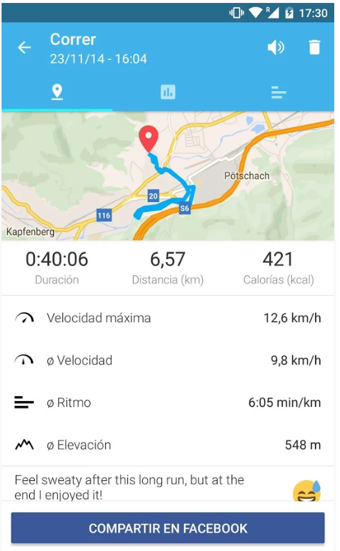
\includegraphics[width=0.3\textwidth]{fitfapp}
                    \caption{Múltiples imágenes de fitfapp}
                    \label{f:fitfapp}
                \end{figure}
                \\\\\textcolor[rgb]{1,0,0}{Aqui va la imagen: imagenes de fitfapp}\\\\
                  \begin{itemize}
                    \item{FUNCIONES DE LA APP}
                    \begin{itemize}
                      \item {Registra la duración, la distancia y el ritmo a través de GPS}
                      \item {Seguimiento de peso y cuenta calorías según tu especificaciones (ayuda a mantener la pérdida de peso)}
                      \item {Comentarios de voz (duración total, calorías, distancia, velocidad actual, ritmo medio)}
                      \item {Función SNAP (toma SNAPS geniales de tus proezas deportivas y comparte con tus amigos)}
                    \end{itemize}
                  \end{itemize}

          \subsubsection{Strava GPS Correr Ciclismo}


                    \begin{figure}[H]
                        \centering
                        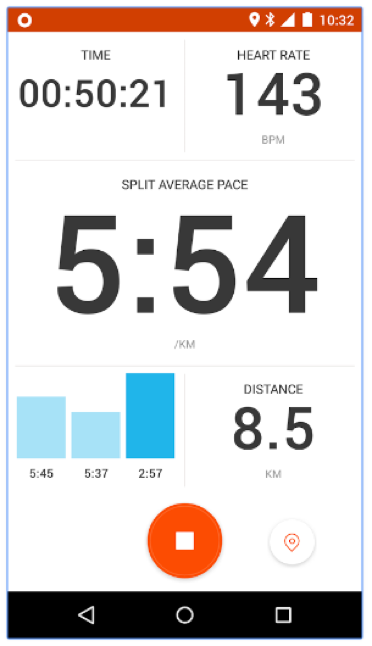
\includegraphics[width=0.3\textwidth]{strava1}
                        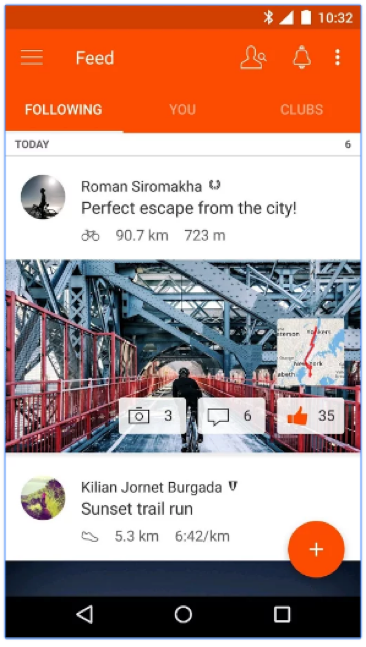
\includegraphics[width=0.3\textwidth]{strava2}
                        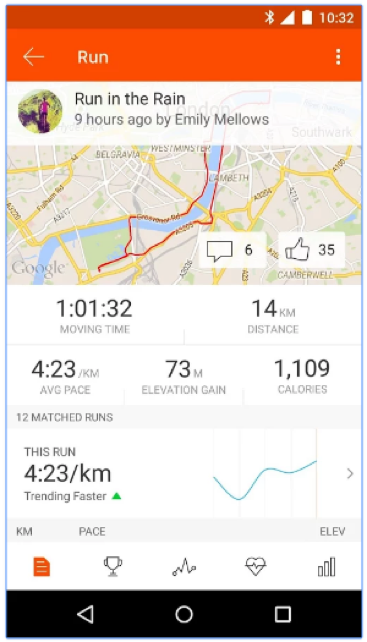
\includegraphics[width=0.3\textwidth]{strava3}
                        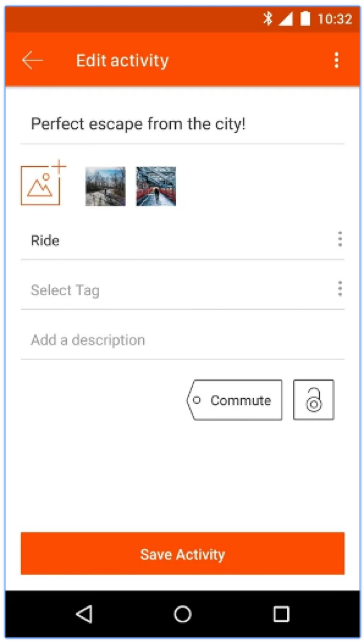
\includegraphics[width=0.3\textwidth]{strava4}
                          \caption{Múltiples imágenes de Strava}
                          \label{f:strava}
                      \end{figure}
                      \\\\\textcolor[rgb]{1,0,0}{Aqui va la imagen: imagenes strava}\\\\
                    \begin{itemize}
                      \item{FUNCIONES DE LA APP}
                      \begin{itemize}
                        \item {Monitoriza gratis las carreras, los recorridos y otras actividades}
                        \begin{itemize}
                          \item {Seguimiento de actividades: Durante la actividad y después de esta, consulta todas las estadísticas importantes como la distancia, el ritmo, la velocidad, el desnivel positivo y las calorías quemadas. También dispondrás de un mapa interactivo de tu actividad.}
                          \item {Reto personal: Participa en los retos personales creados para que superes tus propios límites}
                          \item {Segmentos: ¿Cuál es tu subida de montaña favorita? ¿Y tu tramo de carretera preferido? Mira a ver cómo te ha ido en ciertos momentos de tu actividad con los segmentos de Strava}
                        \end{itemize}
                        \item {Conecta con tus amigos y compañeros}
                        \begin{itemize}
                          \item {Entrenamientos siempre acompañados: Sigue a tus amigos, compañeros de entrenamiento y deportistas profesionales para ver sus actividades y animarlos con los kudos y los comentarios}
                          \item {Clubes: Sea cual sea tu deporte favorito, seguro que existe un club; desde las marcas deportivas más importantes del mundo, hasta tus colegas del barrio con los que sales a correr. Únete a los que más te gusten para no perderte ningún evento, participar en los foros o simplemente para descubrir las últimas novedades}
                          \item {Fotos de las actividades: Presume de los mejores momentos de tu carrera o recorrido en bici}
                          \item {Competición por diversión: Dalo todo y consigue la mejor marca de tiempo en las tablas de resultados de segmentos}
                          \item {Strava y las redes sociales: Comparte todos los detalles de las actividades en Facebook, Instagram y Twitter}
                        \end{itemize}
                        \item {Utiliza tu tecnología favorita}
                        \begin{itemize}
                          \item {Compatible con la mayoría de dispositivos: Strava funciona con la mayoría de dispositivos con GPS incorporado, entre los que se incluyen los relojes para corredores, los ordenadores para ciclistas y los monitores de actividades.}
                          \item {Ritmo cardíaco: Entrena con un monitor de ritmo cardíaco para obtener más datos sobre tu rendimiento.}
                          \item {Android Wear: Gracias a los relojes Android Wear 2.0, ya no necesitarás tu teléfono móvil para registrar y subir una actividad de Strava.}
                        \end{itemize}
                      \end{itemize}
                \end{itemize}

          \subsubsection{RunKeeper - GPS Correr Caminar}
              %   \includegraphics{{runkeeper1}}\includegraphics{{runkeeper2}}\includegraphics{{runkeeper3}}\includegraphics{{runkeeper4}}\includegraphics{{runkeeper5}}\includegraphics{{runkeeper6}}

                  \begin{figure}[H]
                      \centering
                      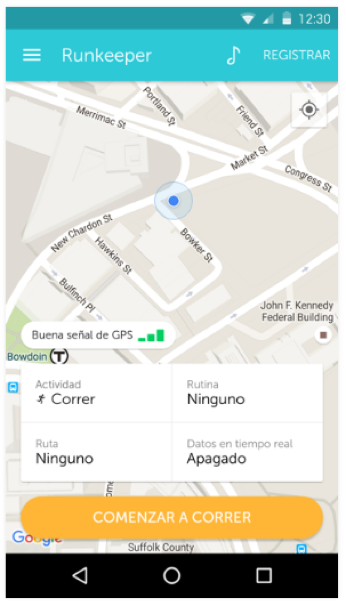
\includegraphics[width=0.3\textwidth]{runkeeper1}
                      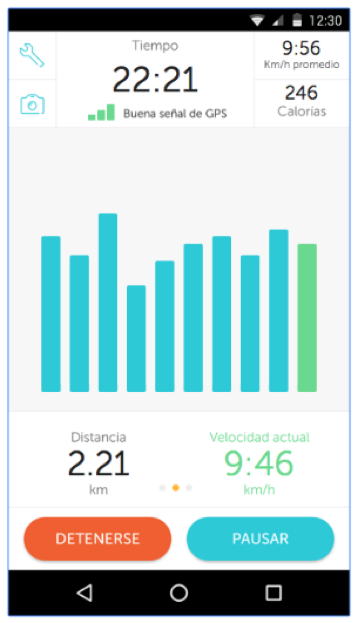
\includegraphics[width=0.3\textwidth]{runkeeper2}
                      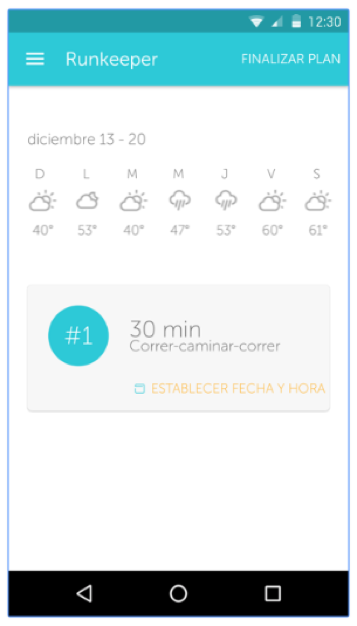
\includegraphics[width=0.3\textwidth]{runkeeper3}
                      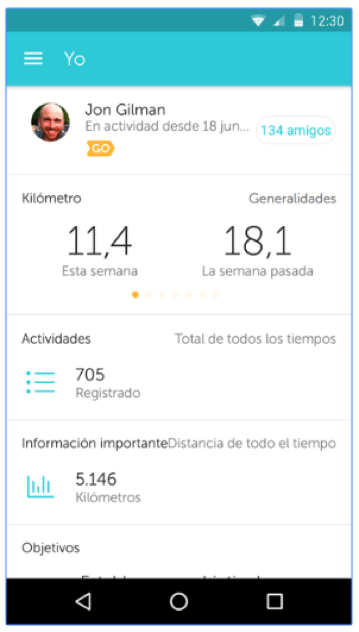
\includegraphics[width=0.3\textwidth]{runkeeper4}
                      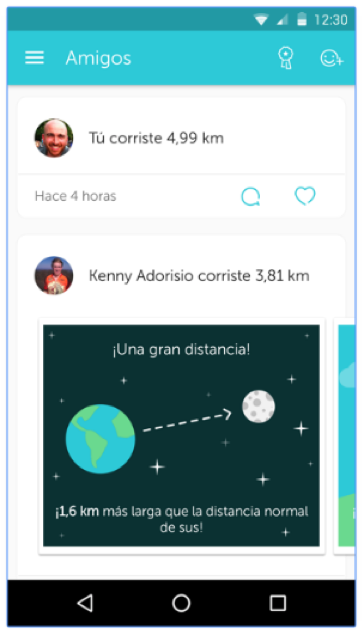
\includegraphics[width=0.3\textwidth]{runkeeper5}
                      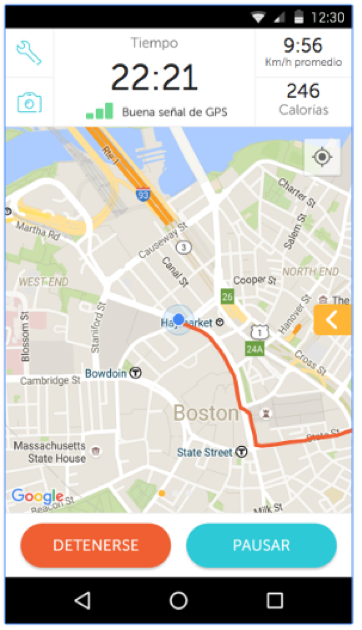
\includegraphics[width=0.3\textwidth]{runkeeper6}
                        \caption{Múltiples imágenes de Runkeeper}
                        \label{f:runkeeper}
                    \end{figure}
                    \\\\\textcolor[rgb]{1,0,0}{Aqui va la imagen: imagenes runkeeper}\\\\
                  \begin{itemize}
                    \item{FUNCIONES DE LA APP}
                    \begin{itemize}
                      \item {Monitoriza tus actividades deportivas y diviértete haciéndolo}
                      \begin{itemize}
                        \item {Verás estadísticas detalladas de tu ritmo, distancia y tiempoVerás estadísticas detalladas de tu ritmo, distancia y tiempo}
                        \item {Obtén estadísticas, progreso y entrenamiento por voz a través de tus auriculares}
                        \item {Toma fotos durante el entrenamiento y compártelas mientras tanto.}
                      \end{itemize}
                      \item {Mide la evolución de tu rendimiento}
                      \begin{itemize}
                        \item {Historial detallado de tus actividades para ver como lo estás haciendo.}
                        \item {Notificaciones cuando consigues nuevas marcas personales e hitos.}
                        \item {Mide tus progresos para conseguir tus objetivos y metas.}
                        \item {Sigue detallados planes de entrenamiento para conseguir objetivos deportivos específicos.}
                        \item {Convierte cualquier actividad en una ruta para poder realizarla más adelante.}
                      \end{itemize}
                      \item {Comparte con amigos}
                      \begin{itemize}
                        \item {Publica tus actividades , logros y planes en para que los vean tus amigos de Facebook, Twitter}
                        \item {Permite que tus fans vean en directo sobre mapas tus entrenamientos y carreras mientras los llevas a cabo (se necesita suscripción a RunKeeper Elite)}
                      \end{itemize}
                      \item {Obtén una visión más amplia de tu salud en RunKeeper.com}
                      \begin{itemize}
                        \item {Integra los datos de tu actividad con más de 70 aplicaciones y servicios de terceros incluyendo , Withings, Zeo, Garmin y muchos más, para conseguir una conocimiento más profundo de tu salud general}
                      \end{itemize}
                    \end{itemize}
                    \subsubsection{Corre con Map My Run}
                      %   \includegraphics{{mapmy1}}\includegraphics{{mapmy2}}\includegraphics{{mapmy3}}

                      \begin{figure}[h]
                          \centering
                          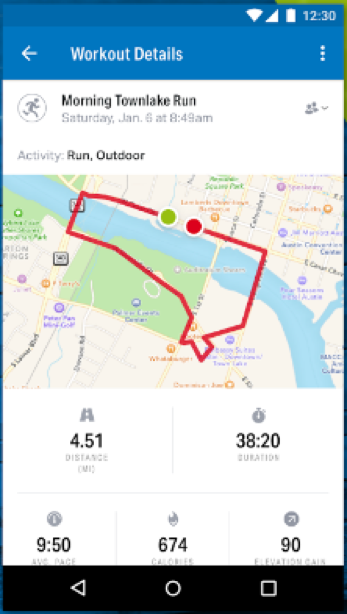
\includegraphics[width=0.3\textwidth]{mapmy1}
                          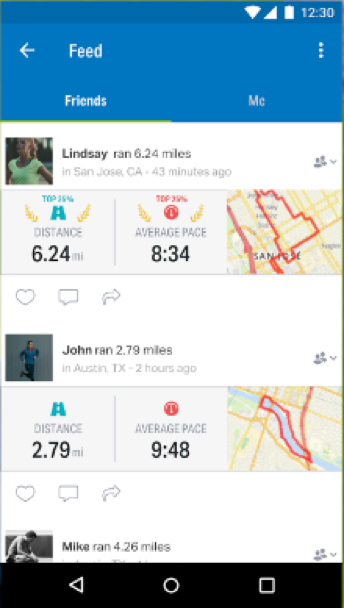
\includegraphics[width=0.3\textwidth]{mapmy2}
                          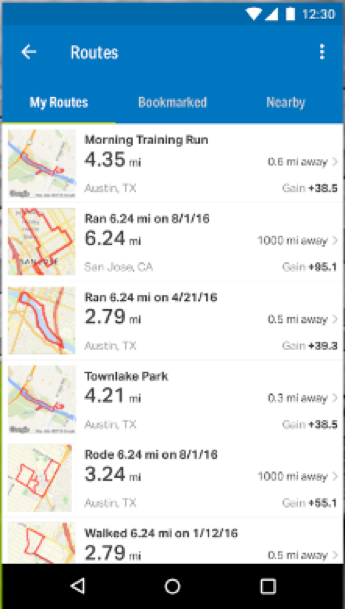
\includegraphics[width=0.3\textwidth]{mapmy3}
                            \caption{Múltiples imágenes de MapMy}
                            \label{f:mapmy}
                        \end{figure}
                        \\\\\textcolor[rgb]{1,0,0}{Aqui va la imagen: Multiples imagenes de Mapmy}\\\\
                          \begin{itemize}
                            \item{FUNCIONES DE LA APP}
                            \begin{itemize}
                              \item {Sigue y sit'ua en el mapa tus entrenamientos}
                              \begin{itemize}
                                \item {Registra además más de 600 actividades deportivas como, por ejemplo, montar en bicicleta, entrenamientos en gimnasio, cross training o yoga.}
                                \item {Obtén información audio en cada entrenamiento que sigas mediante GPS con comentarios de voz personalizables (ritmo, distancia, calorías o desnivel).}
                                \item {Conecta más de 400 dispositivos, importa y analiza información, y almacénala en un solo lugar.}
                                \item {Conecta tus zapatillas y sigue tus kilómetros automáticamente. Recibirás una notificación cuando sea el momento de cambiarlas para evitar lesiones.}
                                \item {Utiliza la función Rutas para encontrar nuevos lugares por los que correr.}
                              \end{itemize}
                              \item {Conecta otras apps y dispositivos}
                              \begin{itemize}
                                \item {Sigue tu actividad con la app Android Wear y consulta tu progreso a simple vista.}
                                \item {Deja que las zapatillas UA Record Equipped sigan de manera automática tu actividad y sincronicen la información con la app.}
                                \item {Sincroniza tu información con las mejores apps y dispositivos como Google Fit, Android Wear, Garmin, Fitbit o Jawbone, entre otros.}
                                \item {Controla tu consumo calórico con MyFitnessPal.}
                              \end{itemize}
                              \item {Únete a la comunidad}
                              \begin{itemize}
                                \item {Consulta la actividad de tus amigos en el Feed y mantén la motivación.}
                                \item {Comparte tus entrenamientos en Facebook y Twitter.}
                                \item {Únete a desafíos para competir con otros usuarios, subir puestos en la clasificación y ganar magníficos premios.}
                              \end{itemize}
                            \end{itemize}
              \end{itemize}

    \section{Herramientas utilizadas}

        \subsection{Introducción}\\
          %\begin{itemize}

              En nuestros días la mejora en los navegadores internos de los dispositivos está haciendo
              posible el auge de aplicacionoes híbridas multiplataforma, acercándolas cada día mas a
              la experiencia y rendimiento de las aplicaciones nativas pero con la ventaja de ser
              implementadas una única vez.\\


              Este tipo de tecnologias nos permiten crear aplicaciones moviles con tecnologia web
              (CSS, HTML y JS) que pueden ser ejecutadas y distribuidas en el market de cada plataforma.\\

              Lo que aporta Ionic es un SDK que facilita la construcción de pantallas (botones, listas, …)
              respetando la guía de estilo de cada plataforma, de forma transparente al desarrollador,
              es decir, que inicialmente no tenemos que añadir una sola línea de código para conseguirlo.\\

              Esta tecnología no es nueva y siempre ha estado ligada con el framework AngularJS y Apache
              Cordova, aquí tenéis un tutorial en el que ya hablábamos de estas tecnologías.\\

              Así que este trinomio se ha seguido manteniendo con la versión 2 de Angular, que como ya
              vimos en este otro tutorial mejora significativamente la productividad de los equipos a
              la hora de desarrollar cualquier tipo de aplicación.\\

              La versión 1 de Ionic ofrecía su SDK como un conjunto de directivas de AngularJS, así que
              está versión 2 hace lo mismo pero con componentes, lo que mejora significativamente el
              rendimiento de su antecesor.\\

              Un punto crítico a la hora de adoptar este tipo de tecnologías es la compatibilidad con
              los distintos dispositivos en sus distintas versiones y plataformas; sobre todo si tiene
              o no compatibilidad con dispositivos antiguos, por aquello de no dejar “colgados” a un
              número significante de usuarios.\\

              En este punto os puedo decir, después de muchas pruebas empíricas, que este tipo de
              tecnologías funcionan perfectamente (sin hacer ninguna configuración adicional) en
              versiones iguales o superiores a la 4.4 de Android, a la 8.0 de IOS y en Windows 10.\\

              En caso de necesitar compatibilidad con versiones 4.2 y 4.3 de Android, se puede
              añadir el plugin de Crosswalk a través de Cordova, que añade un navegador “moderno”
              a nuestra aplicación para que pueda ejecutarse en estas versiones antiguas.
              La única pega es que el tamaño de la aplicación aumenta considerablemente, hemos
              probado con una aplicación de 4 Mb, y el APK ha pasado a 25 Mb y una vez
              instalada ocupa 35 Mb; así que puede ser una buena solución si el espacio no es
              un problema y avisamos fehacientemente al usuario que descargue la aplicación a
              través de una red Wifi. Pero ya os digo esto solo afectaría a dispositivos 4.2 y
              4.3 de Android. Aquí tenéis más información sobre el proyecto crosswalk.\\

              Para Windows el equipo de Ionic considera que no merece la pena mantener compatibilidad
              con versiones anteriores a Windows 10. Esto viene motivado por la poca cuota de mercado
              y a la mejora drástica, en rendimiento y compatibilidad, del navegador en su versión 10.\\

              En conclusión esta tecnología es muy valida siempre que se impongan al cliente ciertas
              restricciones en las versiones de los dispositivos soportados. Android 4.4+, IOS 8+ y
              Windows 10+ (Phone y Desktop).

              %(https://www.adictosaltrabajo.com/tutoriales/empezando-con-ionic-2/).

          %\end{itemize}

        \subsection{HTML5}\\

            Usado para estructurar y presentar el contenido para la web. Es la quinta
            revisión del estándar que fue creado en 1990. La W3C la recomendó para
            transformarse en el estándar a ser usado en el desarrollo de proyectos
            venideros. Con HTML5, tenemos otras posibilidades para explotar usando
            menos recursos. También entra en desuso el formato XHTML, dado que ya no
            sería necesaria su implementación.\\

            HTML5 es un sistema para formatear el layout de nuestras páginas, así como
            hacer algunos ajustes a su aspecto. Con HTML5, los navegadores pueden
            saber cómo mostrar una determinada página web, saber dónde están los
            elementos, dónde poner las imágenes, dónde ubicar el texto. En este
            sentido, el HTML5 no se diferencia demasiado de su predecesor, un lenguaje
            del cual hablamos hace algunos meses en nuestra guía básica de HTML. La
            diferencia principal, sin embargo, es el nivel de sofisticación del código
            que podremos construir usando HTML5.

        \subsection{CSS}\\

          Hojas de estilo en cascada o CSS, es un lenguaje de diseño gráfico para
          definir y crear la presentación de un documento estructurado escrito en un
          lenguaje de marcado.​ Es muy usado para establecer el diseño visual de las
          páginas web, e interfaces de usuario escritas en HTML o XHTML; el lenguaje
          puede ser aplicado a cualquier documento XML, incluyendo XHTML, SVG, XUL,
          RSS, etcétera. También permite aplicar estilos no visuales, como las hojas
          de estilo auditivas.\\

          Junto con HTML y JavaScript, CSS es una tecnología usada por muchos sitios
          web para crear páginas visualmente atractivas, interfaces de usuario para
          aplicaciones web, y GUIs para muchas aplicaciones móviles.\\​

          CSS está diseñado principalmente para marcar la separación del contenido
          del documento y la forma de presentación de este, características tales
          como las capas o layouts, los colores y las fuentes. Esta separación
          busca mejorar la accesibilidad del documento, proveer más flexibilidad y
          control en la especificación de características presentacionales, permitir
          que varios documentos HTML compartan un mismo estilo usando una sola hoja
          de estilos separada en un archivo .css, y reducir la complejidad y la
          repetición de código en la estructura del documento.

          \subsection{TypeScript}\\

          TypeScript es un lenguaje de programación libre y de código abierto
          desarrollado y mantenido por Microsoft. Es un superconjunto de JavaScript,
          que esencialmente añade tipado estático y objetos basados en clases.
          Typescript puede ser usado para
          desarrollar aplicaciones JavaScript que se ejecutarán en el lado del
          cliente o del servidor (NodeJS).\\

          TypeScript extiende la sintaxis de JavaScript, por tanto cualquier código
          JavaScript existente debería funcionar sin problemas. Está pensado para
          grandes proyectos, los cuales a través de un compilador de TypeScript se
          traducen a código JavaScript original.\\

          TypeScript soporta ficheros de definición que contengan información sobre
          los tipos de librerías JavaScript existentes, similares a los ficheros de
          cabeceras de C/C++ que describen la estructura de ficheros de objetos
          existentes. Esto permite a otros programas usar los valores definidos en
          los ficheros como si fueran entidades TypeScript de tipado estático.
          Existen cabeceras para librerías populares como jQuery, MongoDB y D3.js, y
          los módulos básicos de NodeJS.

        \subsection{Node.js}\\

          NodeJS es un entorno de ejecución para JavaScript construido con el
          motor de JavaScript V8 de Chrome. NodeJS usa un modelo de operaciones E/S
          sin bloqueo y orientado a eventos, que lo hace liviano y eficiente. El
          ecosistema de paquetes de NodeJS, npm, es el ecosistema mas grande de
          librerías de código abierto en el mundo.\\

          La gran fortaleza de NodeJS es su entrono multiplataforma de código
          abierto para el desarrollo de aplicaciones de servidor y redes. Las
          siguientes caracteristicas son las mas importantes a la hora de elegir
          para los arquitectos de software a NodeJS:\\

          \begin{itemize}
            \item{Asincróno y controlado por eventos: todas las API de su
                  biblioteca son asíncronas sin bloqueo. Básicamente, significa
                  que un servidor basado en NodeJS nunca espera que una API
                  devuelva datos. El servidor pasa a la siguente API después de
                  llamarlo y un mecanismo de notificación de eventos de NodeJS
                  ayuda al servidor a obtener una respuesta de la llamado API
                  anterior.}
            \item{Altamente escalable: el mecanismo de eventos ayuda al servidor
                  responder de forma no bloqueante y hace que el servidor sea
                  altamente escalable en comparación con los servidores
                  tradicionales que crean subprocesos limitados para manejar las
                  solicitudes. NodeJS utiliza un único programa de subprocesos y
                  el mismo programa puede proporcionar servicio a un número mucho
                  mayor de solicitudes que los servidores tradicionales como
                  Apache HTTP Server.}
            \item{Sin búfer: las aplicaciones nunca almacenann en búfer ningún
                  dato. Estas aplicaciones simplemente generan los datos en
                  fragmentos.}
            \item{Muy rápido: al estar creado en el motor de JavaScript V8 de
                  Google Chrome.}
          \end{itemize}

            % https://www.tutorialspoint.com/nodejs/nodejs_introduction.htm

          ¿Cómo sabemos lo bueno que es Node? Pues mirando quienes la usa: Uber,
          NETFLIX, Medium, Wikipedia, Product Hunt, Flipboard, Trello ... Pues
          esto es un indicador pues ellos que tienen de los mejores ingenieros
          han decidido usar esta tecnología y nos da un indirectamente que la
          tecnología funciona en ambiente a gran escala, porque al usar una
          tecnología nueva y esta no es escalable pues frustrará todo tu trabajo.\\

        \subsection{SQL-lite}\\

            A diferencia de los sistema de gestión de bases de datos cliente-servidor,
            el motor de SQLite no es un proceso independiente con el que el programa
            principal se comunica. En lugar de eso, la biblioteca SQLite se enlaza con
            el programa pasando a ser parte integral del mismo. El programa utiliza la
            funcionalidad de SQLite a través de llamadas simples a subrutinas y
            funciones. Esto reduce la latencia en el acceso a la base de datos, debido
            a que las llamadas a funciones son más eficientes que la comunicación entre
            procesos. El conjunto de la base de datos (definiciones, tablas, índices,
            y los propios datos), son guardados como un sólo fichero estándar en la
            máquina host. Este diseño simple se logra bloqueando todo el fichero de
            base de datos al principio de cada transacción.

        \subsection{Gráfica}\\

          De manera general, cuando tenemos una gran cantidad de datos ya sea
          como texto o como tablas, se prefiere tener toda la información lo
          más esquematizada posible y esto se consigue de distintas formas, un
          ejemplo de ello sería un cuadro de mandos, "Los cuadros de mando han
          de presentar sólo aquella información que sean imprescindible, de una
          forma sencilla y por supuesto, sinóptica y resumida." (Según la
          wikipedia: https://es.wikipedia.org/wiki/Cuadro_de_mando). Por ende
          una buena forma de presentar los datos es mediante graficas, que
          dependiendo de cual puede ser muy intuitiva de cara al usuario.\\

          Entre todas las librerías analizadas nos declinamos en usar Chart.js
          pues esta es una poderosa biblioteca de visualización de datos, pero
          sé que puede ser difícil comenzar y obtener un gráfico para mostrar.
          Pero, ¿Qué es Chart.js? es una biblioteca que visualiza datos mediante
          JavaScript, la cual es mantenida por la comunidad y esta disponible
          en GitHub. Es similar a otras bibliotecas como las de Google Charts.
          Aquí mostramos los tipos de graficas que podemos encontrar en su web:\\

              \begin{figure}[H]
                  \centering
                  \subfigure[Barras]{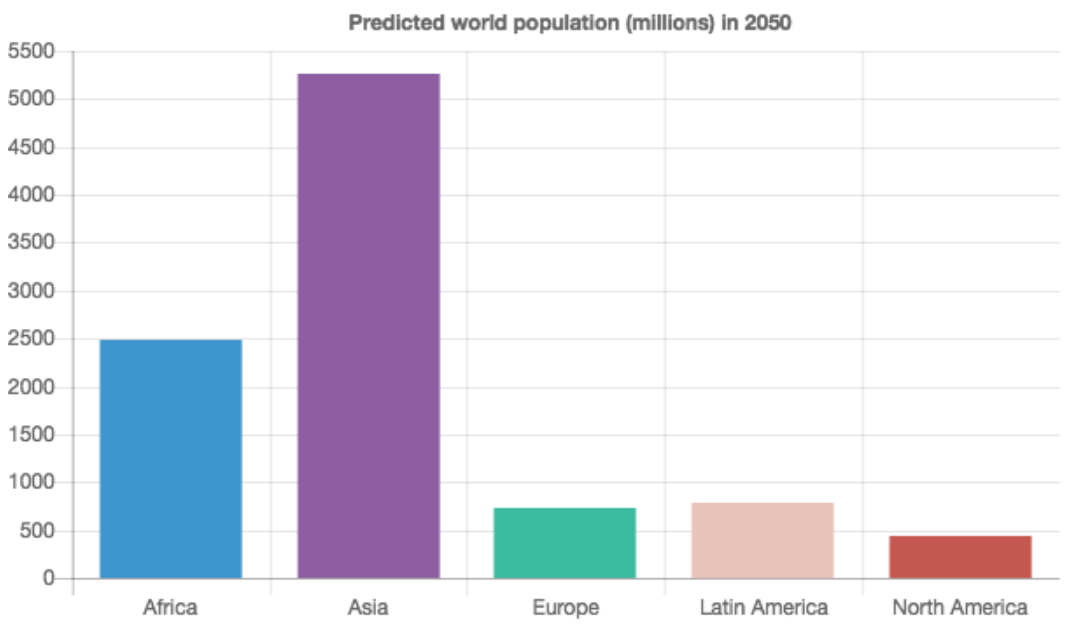
\includegraphics[width=0.48\textwidth]{barras}}
                  \subfigure[Lineas]{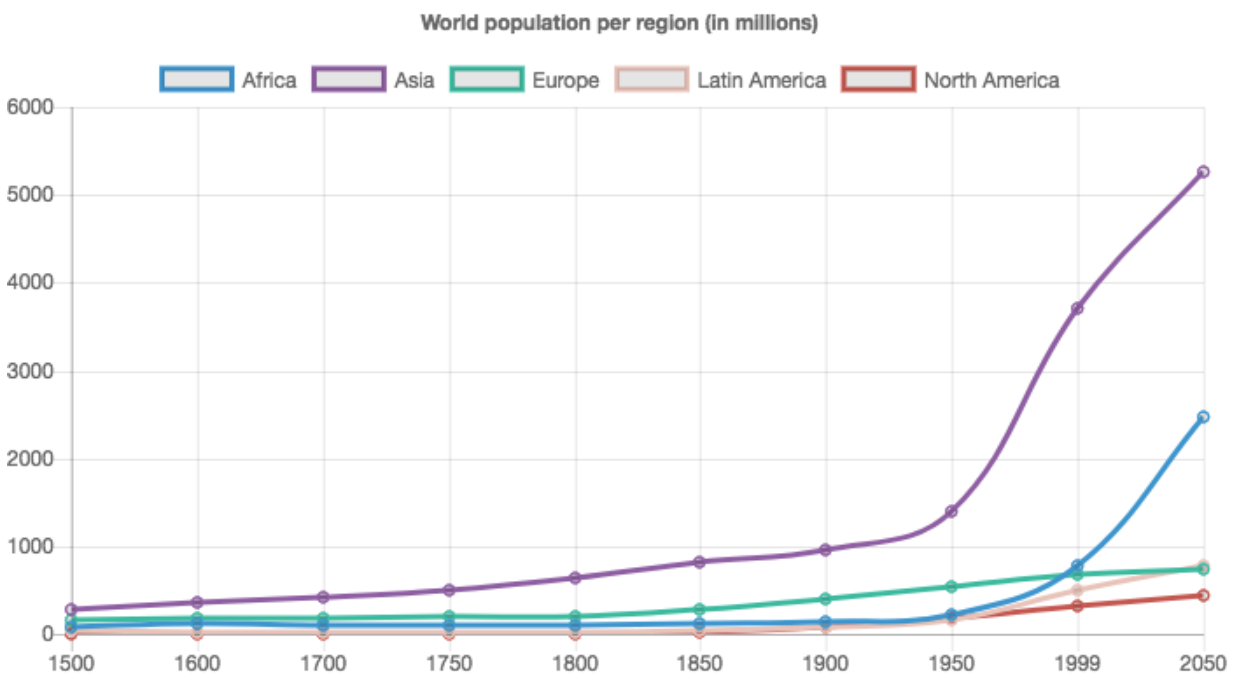
\includegraphics[width=0.48\textwidth]{lineas}}
                  \subfigure[Circular]{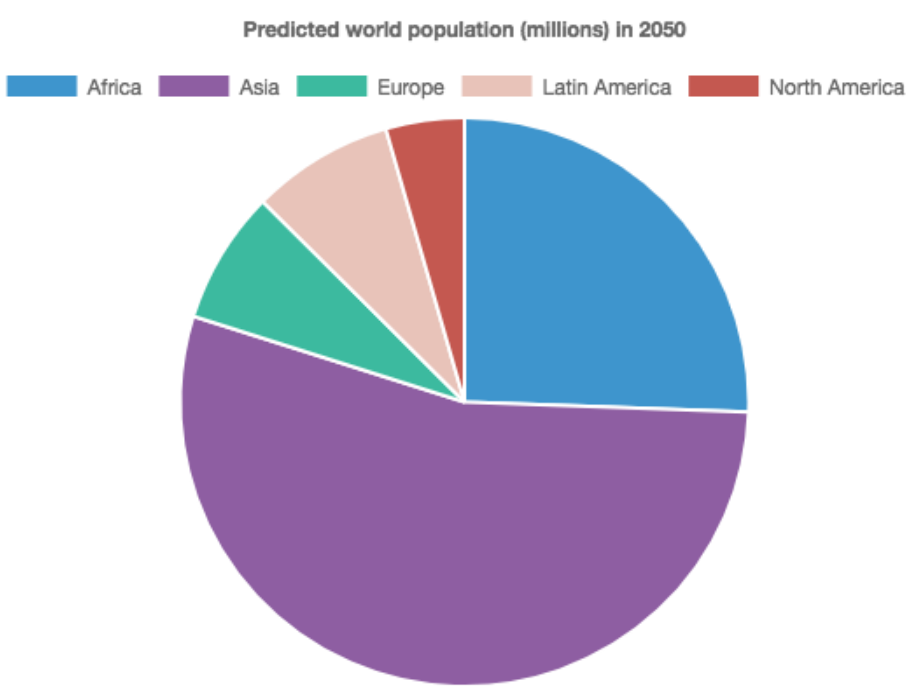
\includegraphics[width=0.48\textwidth]{circular}}
                  \subfigure[Radar]{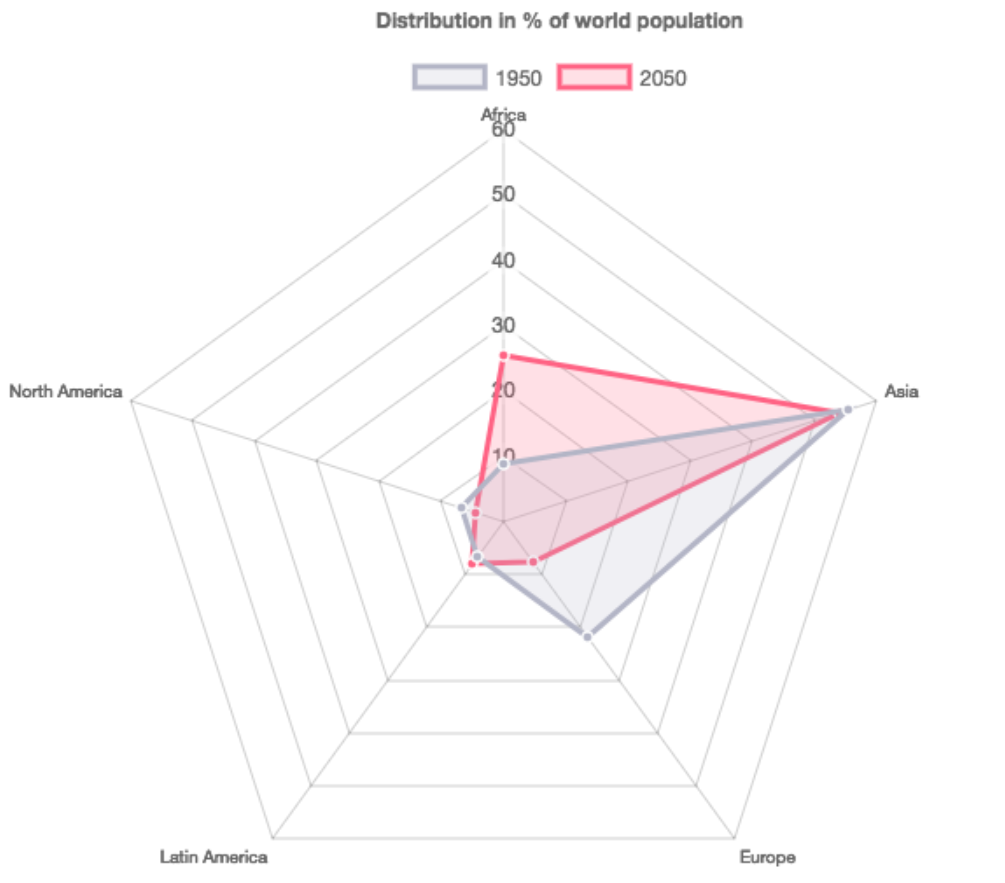
\includegraphics[width=0.48\textwidth]{tabla-radar}}
                  \subfigure[Polar]{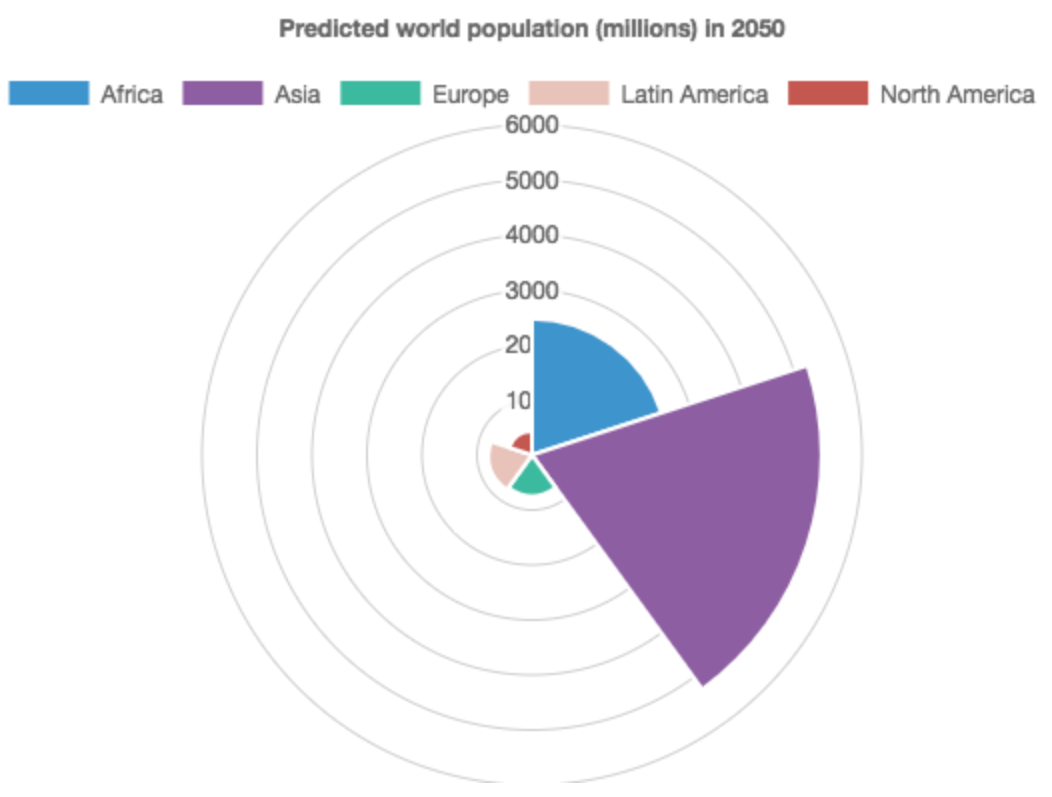
\includegraphics[width=0.48\textwidth]{area-polar}}
                  \caption{Graficas Chart.js (I)}
                  \label{f:chartjsI}
              \end{figure}

              \begin{figure}[H]
                  \centering
                  \subfigure[Rosco]{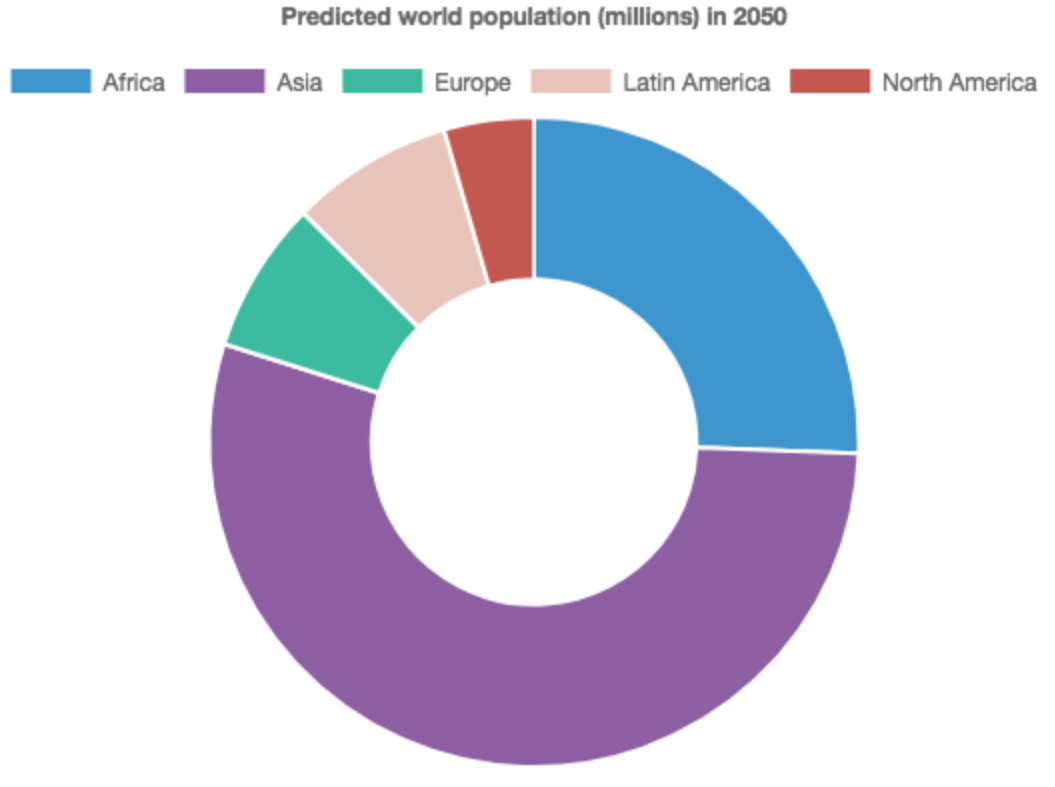
\includegraphics[width=0.48\textwidth]{rosco}}
                  \subfigure[Barras Horizontales]{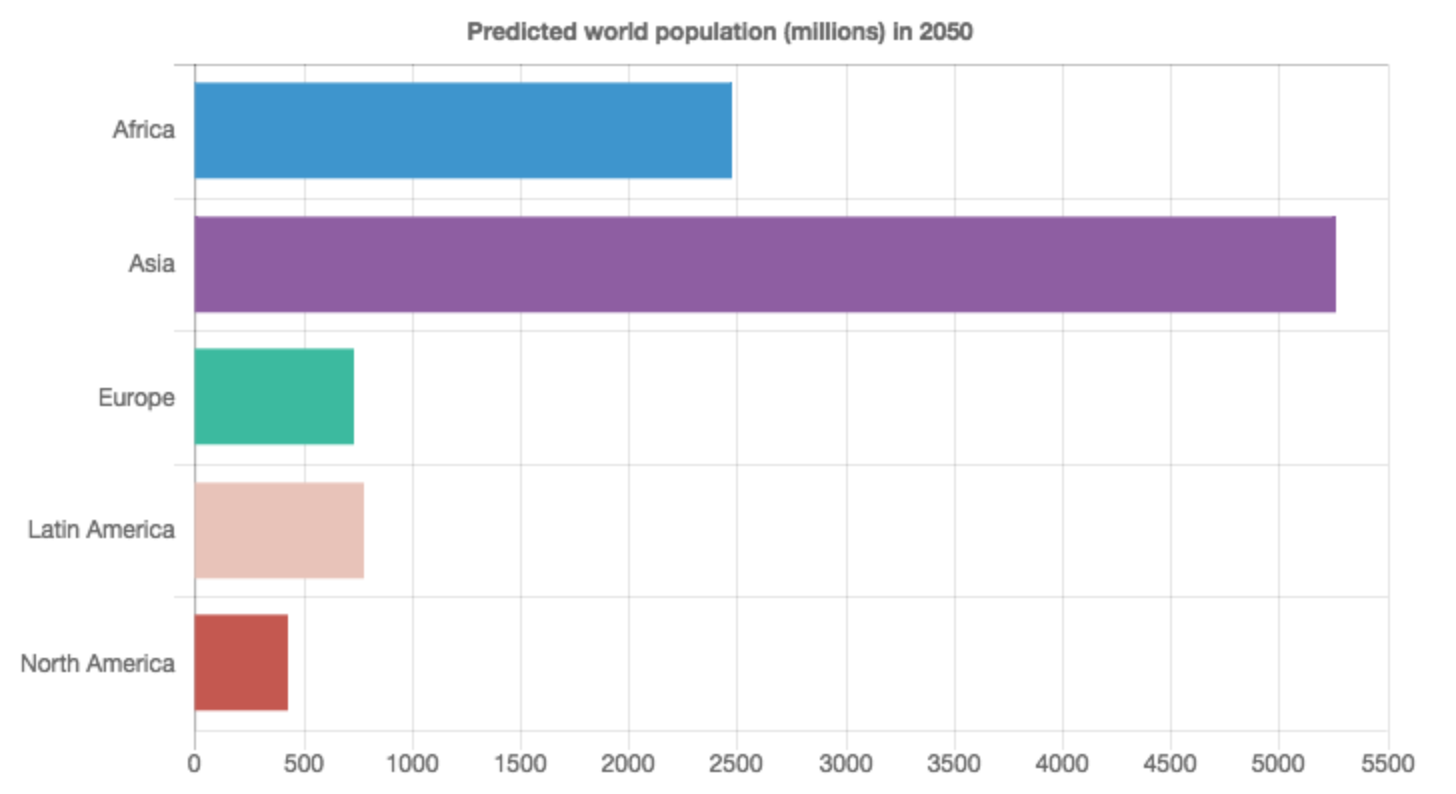
\includegraphics[width=0.48\textwidth]{barras-horizontales}}
                  \subfigure[Barras Agrupado]{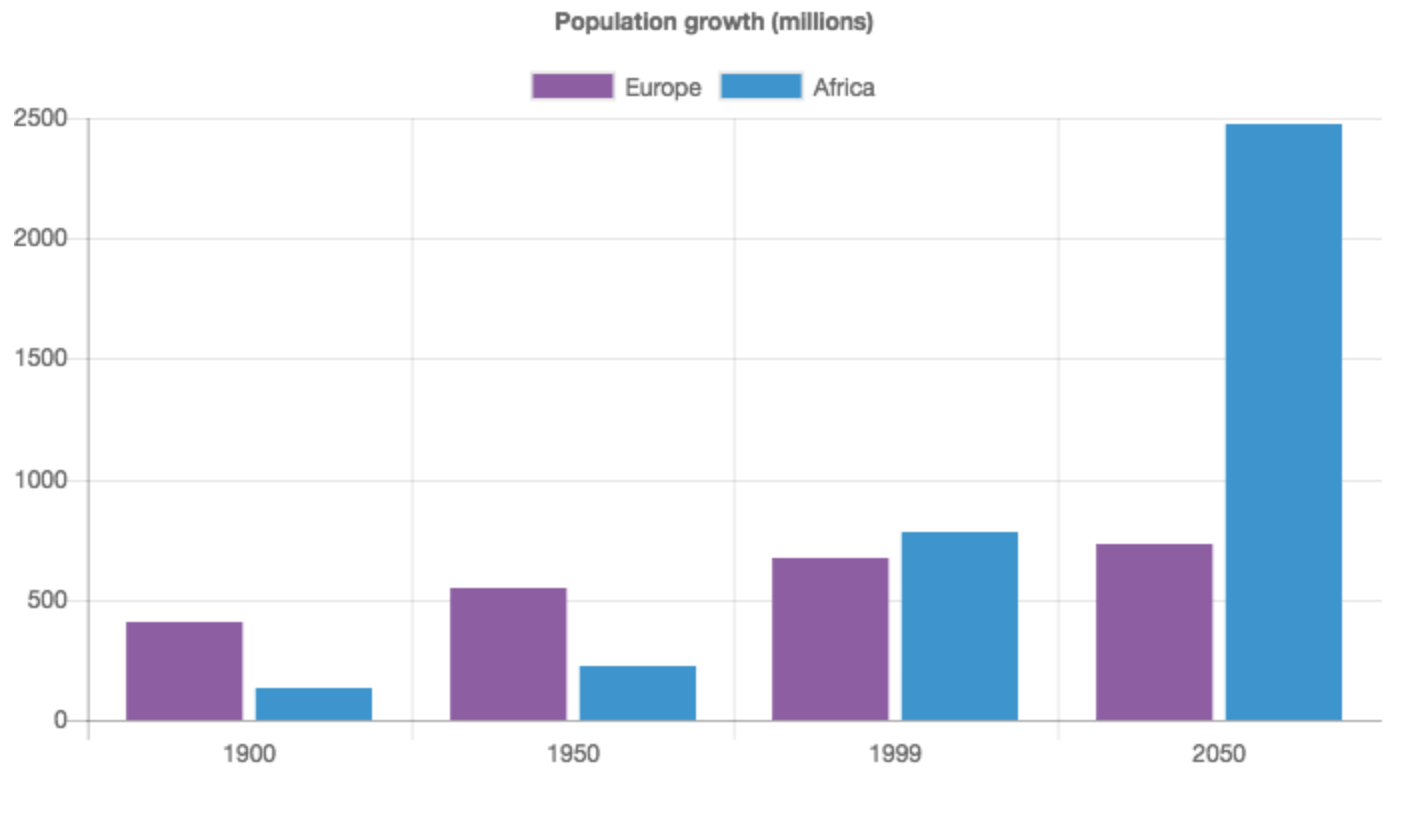
\includegraphics[width=0.48\textwidth]{barras-agrupado}}
                  \subfigure[Cuadro Mixto]{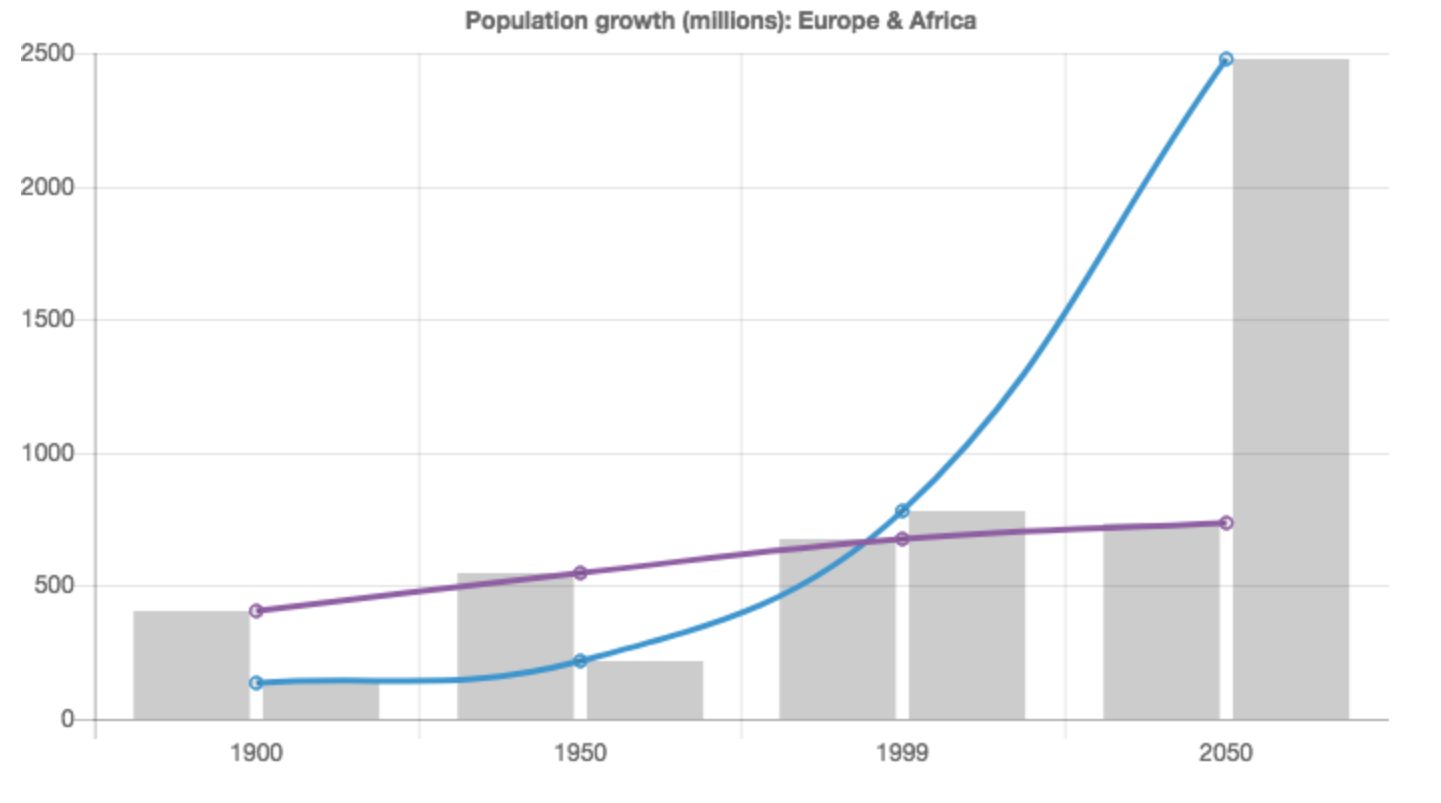
\includegraphics[width=0.48\textwidth]{cuadro-mixto}}
                  \subfigure[Tabla Burbujas]{\includegraphics[width=0.48\textwidth]{tabla-burbujas}}
                  \caption{Graficas Chart.js (II)}
                  \label{f:chartjsII}
              \end{figure}

          Para poder dibujar un gráfico con Chart.js debemos:
          \begin{enumerate}[1.]
            \item Descargar el paquete desde Github.
            \item Definir donde ponerlo en la página web.
            \item Elegir que tipo de gráfico.
            \item Suministrar datos, etiquetas y más.
          \end{enumerate}
          Y ya lo tendremos en nuestro proyecto. Como dato: estos gráficos son muy
          personalizables, como:

          \begin{itemize}
            \item{Estilizar la línea}
            \item{Añadir colores a los distintos elementos. }
            \item{Fuentes}
            \item{Color del área por la llave backgroundColor.}
            \item{dibujar una línea y no rellenarla con ningun color fill}
            \item{Gráficas de linea:}
              \begin{itemize}
                \item{Estilizar la línea}
                \item{Añadir colores a los distintos elementos. }
                \item{Fuentes}
                \item{Color del área por la llave backgroundColor.}
                \item{dibujar una línea y no rellenarla con ningun color fill}
              \end{itemize}
          \end{itemize}

        \subsection{Google Maps}\\

        \subsection{GPS}\\

        \subsection{Angular JS}\\

            La consolidadción del framework más demandado de JavaScript desarrollado
            por el gigante Google, Angular 2, ha sido clave en la creación de Ionic.
            Desde hace un tiempo venimos escuchando hablar mucho de aplicaciones web
            escritas con AngularJS. Muchos o la mayoría ya habréis tenido contacto
            con este Framework o simplemente le habéis echado un ojo sin meteros en
            desarrollo con él. Los que lo estáis usando no podréis negar la
            velocidad de desarrollo que se adquiere en nuestros proyectos y la
            rápida curva de aprendizaje que tiene. No obstante, nunca está de más
            hablar de este Framework MVC para los que aun no lo conocen y como nos
            puede beneficiar a la hora de programar una aplicación con Phonegap.\\

            AngularJS es un framework JavaScript creado y mantenido por Google que es
            utilizado para la creación de aplicaciones web siguiendo el patrón Modelo
            Vista Controlador, capacitado para extender nuestros documentos HTML
            añadiendo nuevas etiquetas y atributos que cumplirán con funciones
            específicas ya definidas o programadas por el desarrollador.\\

            Ventajas de usar AngularJS:
            \begin{itemize}
              \item {Con AngularJS tendrás tu código JavaScript organizado.}
              \item {Desarrollo más rápido.}
              \item {Es compatible con JQuery y otras librerías (con el uso veremos que
                     con AngularJS es suficiente para manipular el DOM).}
              \item {Facilidad para hacer tests.}
            \end{itemize}

            Desarrollando con AngularJS
            Según empezamos con AngularJS, aprenderemos diferentes conceptos como son
            módulos, controladores, directivas, expresiones, filtros, etc… que nos
            permitirán realizar muchas funcionalidades con un menor esfuerzo, así como
            organizar nuestro código y poder mantenerlo limpio y entendible. Veremos
            con qué facilidad se referencian los datos que tenemos en los modelos a
            las vistas, así como la organización del funcionamiento de cada vista con
            su propio controlador. Podremos separar nuestro código en módulos para
            facilitar su organización e incluso poder exportarlo a otros proyectos.

            %(http://www.phonegapspain.com/que-es-y-como-empezar-con-angularjs/)

        \subsection{Ionic}\\

            Ionic es un framework para el desarrollo de aplicaciones híbridas,
            su directriz inicial era pensado en los smartphones (formato móviles y
            tablets), pero también es posible su uso para implementar aplicaciones
            web. Su característica fundamental es que usa por debajo corodova y
            Angular 2, ademas de otras componentes, que facilitando así el
            desarrollo.\\

            Pensada para obtener resultados de una manera rápida y con una menor
            inversión económica, ya que permite crear aplicaciones para distintas
            plataformas móviles con una misma base de código. Estas son:\\

                      \begin{figure}[H]
                        \centering
                        \includegraphics[width=0.9\textwidth]{tablaPlataformasIonic}
                        \caption{Plataformas de Ionic}
                        \label{f:plataformas}
                      \end{figure}
                      \\\\\textcolor[rgb]{1,0,0}{Aqui va la imagen: plataformas de ionic}\\\\

            Hemos mencionado que Ionic desarrolla aplicaciones híbridas, pero ¿Qué
            es una aplicación híbrida?\\

            Es la que nos permite desarrollar mediante las tecnologías web: HTML +
            CSS + Javascript. A la hora de instalarla el dispositivo no ve
            diferencias con una realizada através de Android Studio o Xcode, que
            puedes descargar a través de las tiendas de cada sistema, por lo que en
            principio los usuarios finales no hallarán diferencia con respecto al
            resto de aplicaciones nativas.\\

            Otra de sus grandes ventajas es que al ejecutarse con tecnologías web,
            los desarrolladores expertos en este medio pueden aprovechar dichos
            conocimentos teniendo una adaptación rápida en el desarrollo de apps
            para móviles.\\

            ejecutan en lo que se denomina un “web view”, que no es más que una
            especie de navegador integrado en el móvil y en el que solamente se
            ejecuta la app híbrida.\\

            Las aplicaciones híbridas son interesantes por diversos motivos:
            \begin{itemize}
                \item{Con una misma base de código serán capaces de compilar apps
                para funcionar correctamente en una gran cantidad de sistemas
                operativos de móviles o tablets. Generalmente nos será suficiente
                que nuestra app funcione en iOS y Android, pero Ionic es capaz de
                compilar a otros sistemas como Windows Phone.}
                \item{El coste del desarrollo es sensiblemente menor, ya que no es
                necesario contar con varios equipos de desarrollo para cada lenguaje
                concreto de cada plataforma.}
                \item{El tiempo de desarrollo también es menor, ya que solo es
                necesario construir la aplicación una vez e inmediatamente la
                tendremos en todas las plataformas a las que nos dirigimos.}
                \item {Es de más fácil adaptación para los desarrolladores que
                vienen de la web.}
            \end{itemize}

            Para el desarrollo de una aplicación varia en función del entorno de
            desarrollo. Si queremos desarrollar en windows queda descartada la
            posibilidad de compilación de la app iOS. Pero podemos desarrollar en
            windows, para android y para windows phone, y posteriormente exportarlo
            a un macOS y desde este compilarlo en Xcode y obtener las tres
            plataformas mas importantes.\\

            Los requisitos para desarrollar en los distintos SO son:
            \begin{itemize}
                \item{NodeJS}
                \item{Paquetes Cordova e Ionic}
                \item{SDK de Android / Xcode}
                \item{Java JDK (Android)}
                \item{Y sólo para macOS: apache-ant}
            \end{itemize}

            Con ello ya estaremos listos para desarrollar nuestra aplicacón. Para
            empezar a desarrollar es tan simple como ejecutar en el directorio que
            queremos el proyecto: ionic start nombreApp tipoPlantilla -v3\\

            Como vemos en el comando lo primero que tenemos es start para indicarle
            a ionic que queremos iniciar un proyecto, el segundo parametro es el
            nombre de la aplicacion, tercero es el tipo de plantilla que veremos los
            distintos tipos que nos ofrece ionic y por ultimo es la version que
            queremos que se instale, las versiones van desde la uno, pasando por la
            dos y finalizando en la tres.


                   \begin{figure}[H]
                     \centering
                            \subfigure[Android]{\includegraphics[width=0.3\textwidth]{blankA}}
                            \subfigure[iOS]{\includegraphics[width=0.3\textwidth]{blankIOs}}
                            \subfigure[Windows Phone]{\includegraphics[width=0.3\textwidth]{blankWP}}
                      \caption{Tipo de plantilla: blank}
                      \label{f:blank}
                    \end{figure}


                  \begin{figure}[H]
                    \centering
                           \subfigure[Android]{\includegraphics[width=0.3\textwidth]{tabsA}}
                           \subfigure[iOS]{\includegraphics[width=0.3\textwidth]{tabsIOS}}
                           \subfigure[Windows Phone]{\includegraphics[width=0.3\textwidth]{tabsWP}}
                     \caption{Tipo de plantilla: tabs}
                     \label{f:tabs}
                   \end{figure}


                 \begin{figure}[H]
                   \centering

                        \subfigure[Android]{\includegraphics[width=0.3\textwidth]{sidemenuA}}
                        \subfigure[iOS]{\includegraphics[width=0.3\textwidth]{sidemenuIOS}}
                        \subfigure[Windows Phone]{\includegraphics[width=0.3\textwidth]{sidemenuWP}}
                  \caption{Tipo de plantilla: sidemenu}
                  \label{f:blank}
                \end{figure}

            Esto permite iniciar de manera rapida un proyecto y con un diseño en la
            interfaz de nuestra app. Dicha interfaz se observa que guarda una
            disposicion ordenada y limpia. La manera de usar los elementos como los
            iconos, la letra o la disposición de los mismos, varía dependiendo de la
            plataforma a utilizar, como hemos visto en las imagenes anteriores.\\

            Retomando el tema de las versiones vemos diferencias en su estructura,
            de un simple vistazo vemos:

              \begin{figure}[H]
                \centering
                     \subfigure[Ionic v1]{\includegraphics[width=0.3\textwidth]{estructuraV1}}
                     \subfigure[Ionic V2-v3]{\includegraphics[width=0.3\textwidth]{estructuraV2V3}}
                     \caption{Estructura en proyecto Ionic}
                     \label{f:estructura}
              \end{figure}
              \\\\\textcolor[rgb]{1,0,0}{Aqui va la imagen: Estructura en proyecto Ionic}\\\\
            Ahora vamos a describir los distintos
            \begin{itemize}
                \item{hooks: Son scripts que se disparan durante el proceso de
                      construcción. Generalmente se usan por comandos de Cordova
                      para customización y la construcción de procesos automáticos.}
                \item{platforms: Aquí es donde se crean los proyectos de Android y
                      de IOS. Podemos encontrarnos algunos problemas específicos de
                      la plataforma durante el desarrollo que requieren estos
                      archivos. Pero las dejaremos intactas durante la mayor parte
                      del tiempo.}
                \item{plugins: Aquí se encuentran los plugins de Cordova. Cuando se
                      crea una aplicación de Ionic, ya hay algunos de estos plugins
                      instalados.}
                \item{resources: Esta carpetas se utiliza para añadir recursos como
                      el icono y la pantalla de bienvenida.}
                \item{scss: Desde que el núcleo de Ionic esta construido con Sass,
                      está es la carpeta donde se encuentra el archivo.}
                \item{www:  Es la carpeta donde trabajaremos de forma habitual y
                      mantiene una estructura de carpetas en su interior por
                      defecto, pero se pueden modificar según las necesidades del
                      proyecto.}
            \end{itemize}


             \begin{figure}[H]
               \centering
                    \subfigure[Ionic v1]{\includegraphics[width=0.3\textwidth]{wwwV1}}
                    \subfigure[Ionic v2-v3]{\includegraphics[width=0.3\textwidth]{srcV2V3}}
                    \caption{Lugar de trabajo}
                    \label{f:estructuraTrabajo}
              \end{figure}

            \\\\\textcolor[rgb]{1,0,0}{Aqui va la imagen: Lugar de trabajo}\\\\

            Aqui ya vemos el "lugar de trabajo" que empezaremos a describir los
            distintos directorios, de www, en la versión uno:

            \begin{itemize}
                  \item{css: aquí estarán nuestros estilos CSS.}
                  \item{img: para las imágenes.}
                  \item{js: contiene el fichero principal de configuración app.js,
                        los componentes de AngularJS (controladores, servicios,
                        directivas) y todos los archivos js.}
                  \item{libs: aquí pondremos las librerías.}
                  \item{templates: para los archivos html.}
                  \item{index.html: el punto de inicio de la aplicación.}
            \end{itemize}

            Por otro lado tenemos los directorios de src para la versión dos y tres:

            \begin{itemize}
                  \item{app: contiene el fichero principal de configuración app.js,
                        los componentes de AngularJS (controladores, servicios,
                        directivas) y todos los archivos js.}
                  \item{assets: archivos de imágines y otro de materiales externos
                        que vas a usar en las páginas.}
                  \item{pages: se alojaran las páginas que contenga nuestra
                        aplicación.}
                  \item{theme: directorio en el cual se puede hacer cambios en las
                        variables generales de la interfaz de nuestra app.}
            \end{itemize}

            Lo más notorio en estas dos estructuras es el directorio pages que nos
            ofrece las últimas versiones. Gracias a este cambio es mucho más
            intuitivo, en este directorio nos encontramos tres ficheros por cada
            vista que tenga la app, y son:

            \begin{itemize}
                \item{.html: es la necesaria para poder realizar la vista.}
                \item{.css: que nos permite introducir codigo css que será usado por
                       la extension .html.}
                \item{.ts: que se trata del controlador.}
            \end{itemize}

            En la versión uno tenias un sólo fichero typeScript para todas las
            vistas, uno solo para todo el css y otro
            Esto hace que la curva de aprendizaje sea positivamente acelerada.
            Y le digo de buena tinta, ya que he pasado por todas las versiones,
            que este pequeño cambio marca un antes y un despues.\\



            Tambien tenemos dos comandos que son de utilidad para realizar la
            vista de nuestro proyecto y son:

            \begin{itemize}
                \item{ionic serve}
                \item{ionic serve --lab}
            \end{itemize}
            Esto nos permite visualizar en nuestro navegador web, recomendamos

            \subsubsection{Api Google Maps}\\

            \subsection{Api GPS}\\


\section{Análisis y diseños}

       \subsection{Casos de usos}\\

           \begin{figure}[H]
             \centering
                  \includegraphics[width=0.8\textwidth]{CasoDeUso-RealizarCarrera}
                  \includegraphics[width=0.8\textwidth]{CasoDeUso-VisualizarDatos}
            \caption{Caso de uso}
            \label{f:casosdeuso}
          \end{figure}

          \\\\\textcolor[rgb]{1,0,0}{Aqui va la imagen: Caso de uso}\\\\

       \subsection{Escenarios}\\

       \subsection{Diseño de objetos}\\

       \subsection{Programar}\\


\section{Medios Materiales}


        \begin{itemize}
        	\item{Herramientas Hardware:}\\
                         - PCs ímpreso\\
        	         - Impresora
        	\item{Herramientas Software: }\\
                         - Sistema operativo ESPECIFICA \\
                         - Herramientas de edici\'{o}n y de  desarrollo de programas  ESPECIFICA \\
        \end{itemize}


\section{Bibliografía}

      \begin{itemize}
        \item ARTICULO1
        \item ARTICULO2
        \item ARTICULO3
      \end{itemize}


\end{document}
